\section{Simulation and Observations}
\label{section:observations}
In this section we make use of our model by simulating it for various cases. First we will demonstrate some basic dynamics based on the impact of dissipation $\lambda$, desired velocities $u_i$, and interaction $A$. Next we will focus on collective behavior, and present self-organization such as lane and stripe formations for counter and cross flows respectively. Later we will repeat the same experiments with addition of stochastic elements. Some insights are provided on the relationship between the parameters, Hamiltonian, and the collective behavior.

The model parameters defined for the simulation are the same as defined in \autoref{code:model_init}. Any changes made would be mentioned within their respective cases. For reproducibility and comparison, each simulation starts with the same arrangement of pedestrians on the xy-plane as shown below.
\begin{figure}[H]
    \centering
    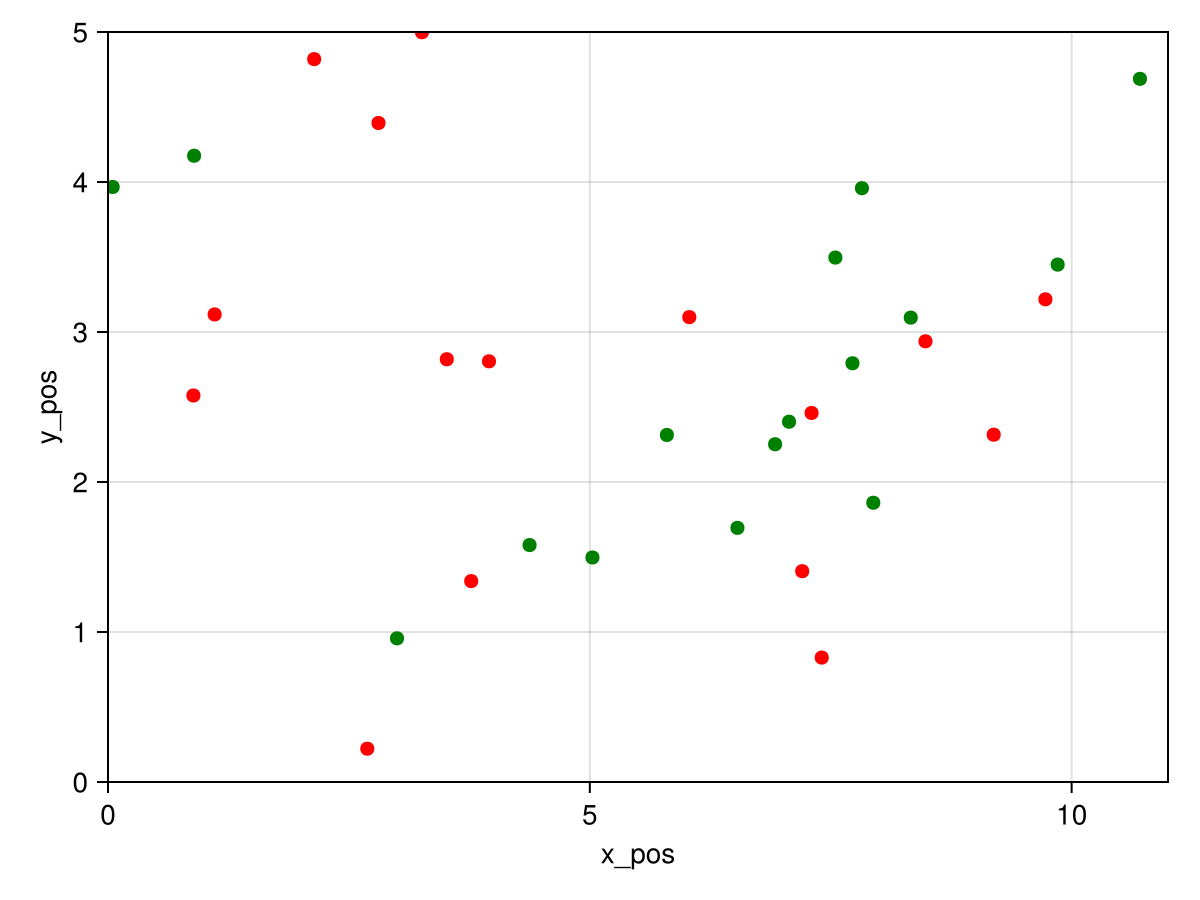
\includegraphics[width=0.55\textwidth]{figures/ch5_basic/start_pos.png}
    \caption{Starting positions of pedestrians.}
    \label{plot:starting_pos}
\end{figure}
The colors in \autoref{plot:starting_pos} distinguishes groups of pedestrians each having same desired speeds. This is only relevant for flows that are multidirectional, as will be shown in \autoref{section:collective}. In the cases of unidirectional flow or where the direction is irrelevant, the color for all is the same.

\subsection{Basic Dynamics}
This section serves to illustrate how the changes in the parameters affect the dynamics of the model, although none of the dynamics presented in the model are realistic, the diagrams provide a way to think about the dynamics of the model based on the changes in the parameter.
\pagebreak
\begin{itemize}
    \item \textbf{No desired velocity ($u_i = \begin{bmatrix} 0 & 0 \end{bmatrix}$) with dissipation ($\lambda > 0$):}
\begin{figure}[H]
    \centering
    \begin{subfigure}{0.49\textwidth}
        \centering
        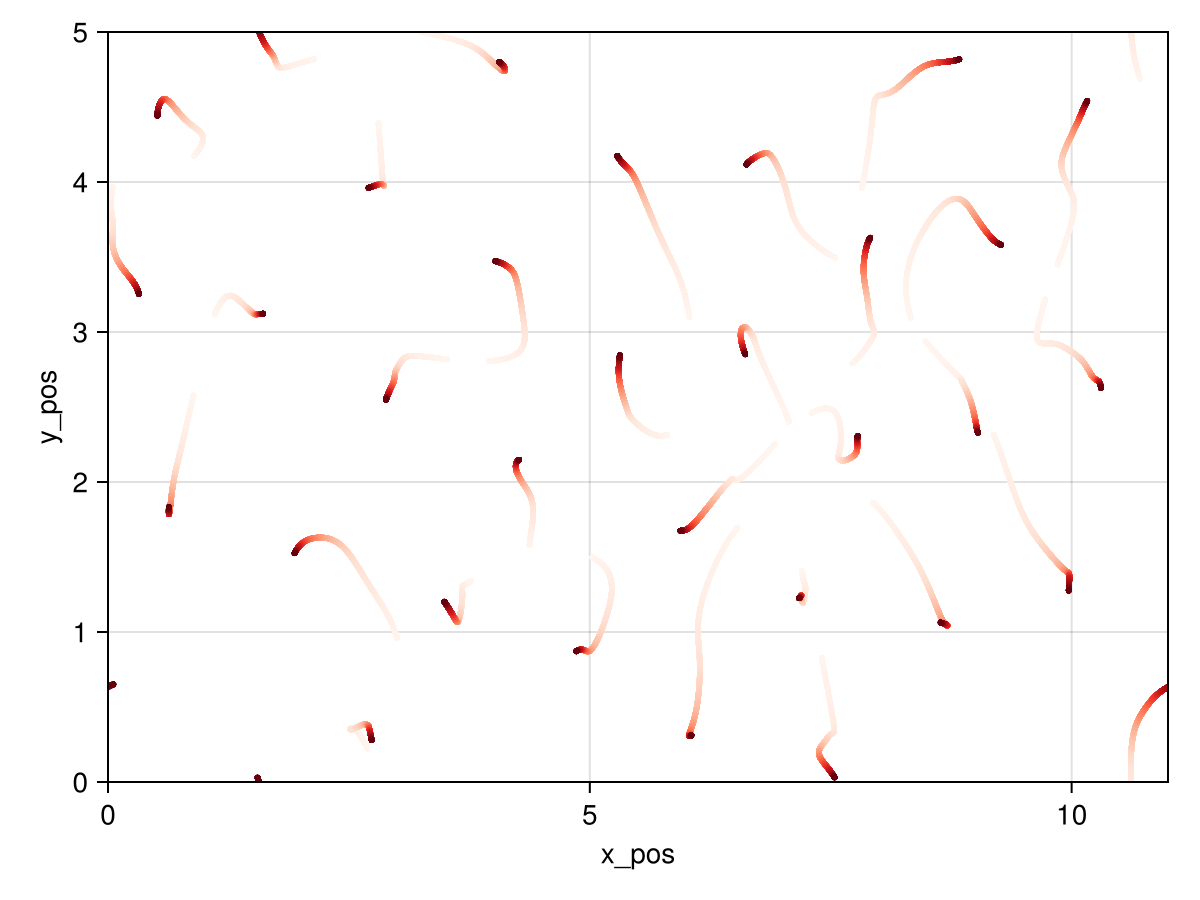
\includegraphics[width=\linewidth]{figures/ch5_basic/traj_crys_4000.png}
        \caption{Pedestrian trajectories}
        \label{plot:crys_traj}
    \end{subfigure}
    \begin{subfigure}{.49\textwidth}
        \centering
        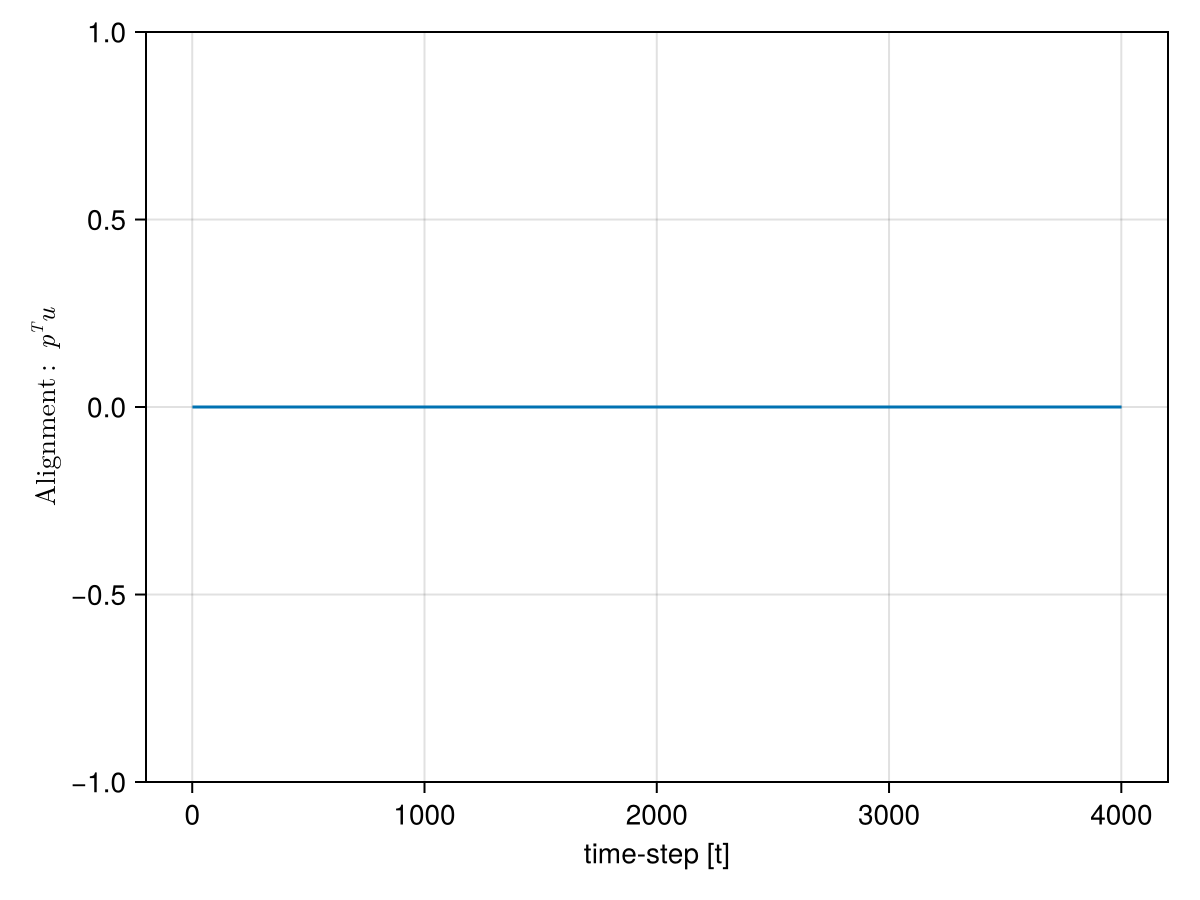
\includegraphics[width=\linewidth]{figures/ch5_basic/straight_crys.png}
        \caption{Alignment}
        \label{plot:crys_alignment}
    \end{subfigure}
    \caption{Crystallization of pedestrians due to no input $u_i = 0$ and allowing the system to dissipate energy}
    \label{plot:crys}
\end{figure}
Allowing the system to dissipate $\lambda > 0$ while simultaneously the pedestrians have no desired velocity \autoref{plot:crys}, essentially creates a system with an active output port, but no input. The results are as expected, the system keeps losing energy leading the pedestrians to crystallize over time. The alignment here is zero, because the desired velocity $u_i = 0$  

\begin{figure}[H]
    \centering
    \begin{subfigure}{0.49\textwidth}
        \centering
        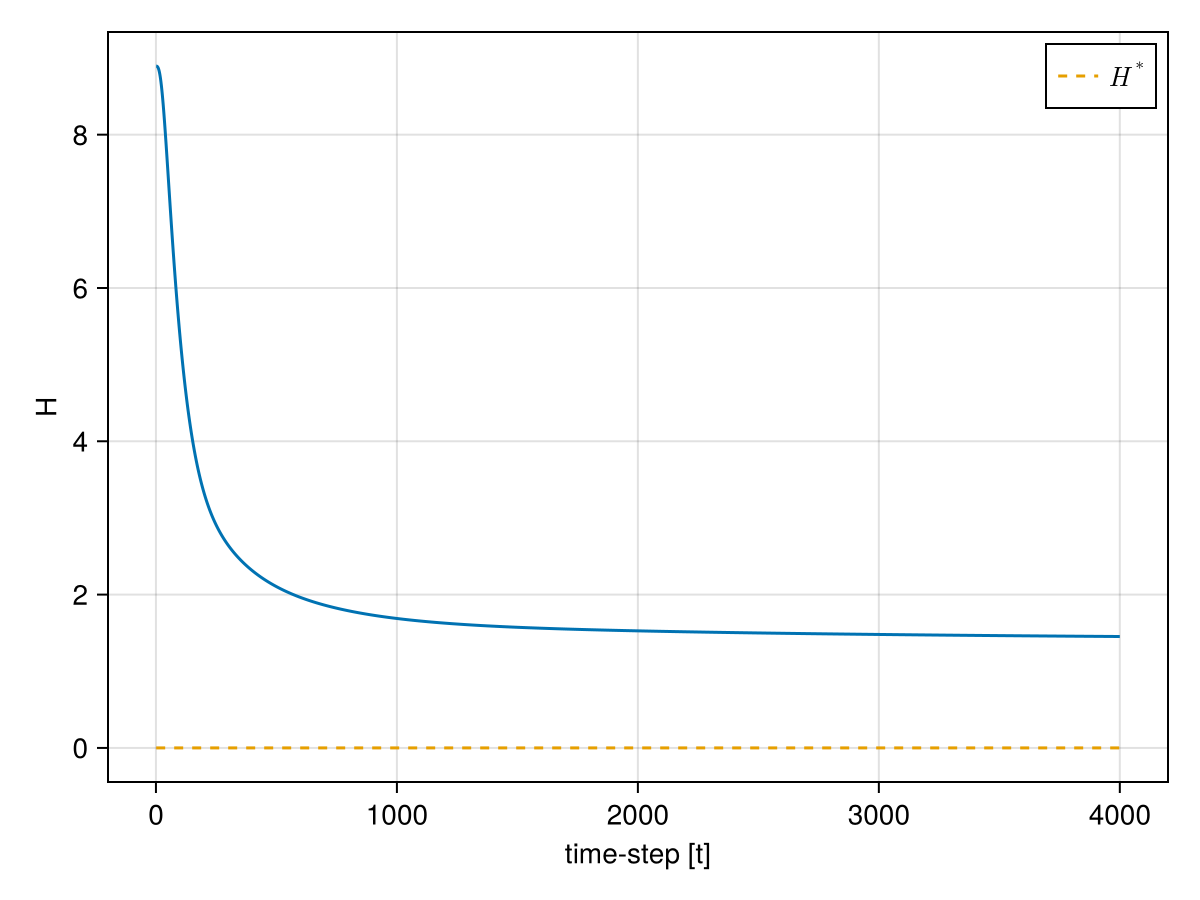
\includegraphics[width=\linewidth]{figures/ch5_basic/H_crys.png}
        \caption{Hamiltonian $H$ over time}
        \label{plot:crys_h}
    \end{subfigure}
    \begin{subfigure}{.49\textwidth}
        \centering
        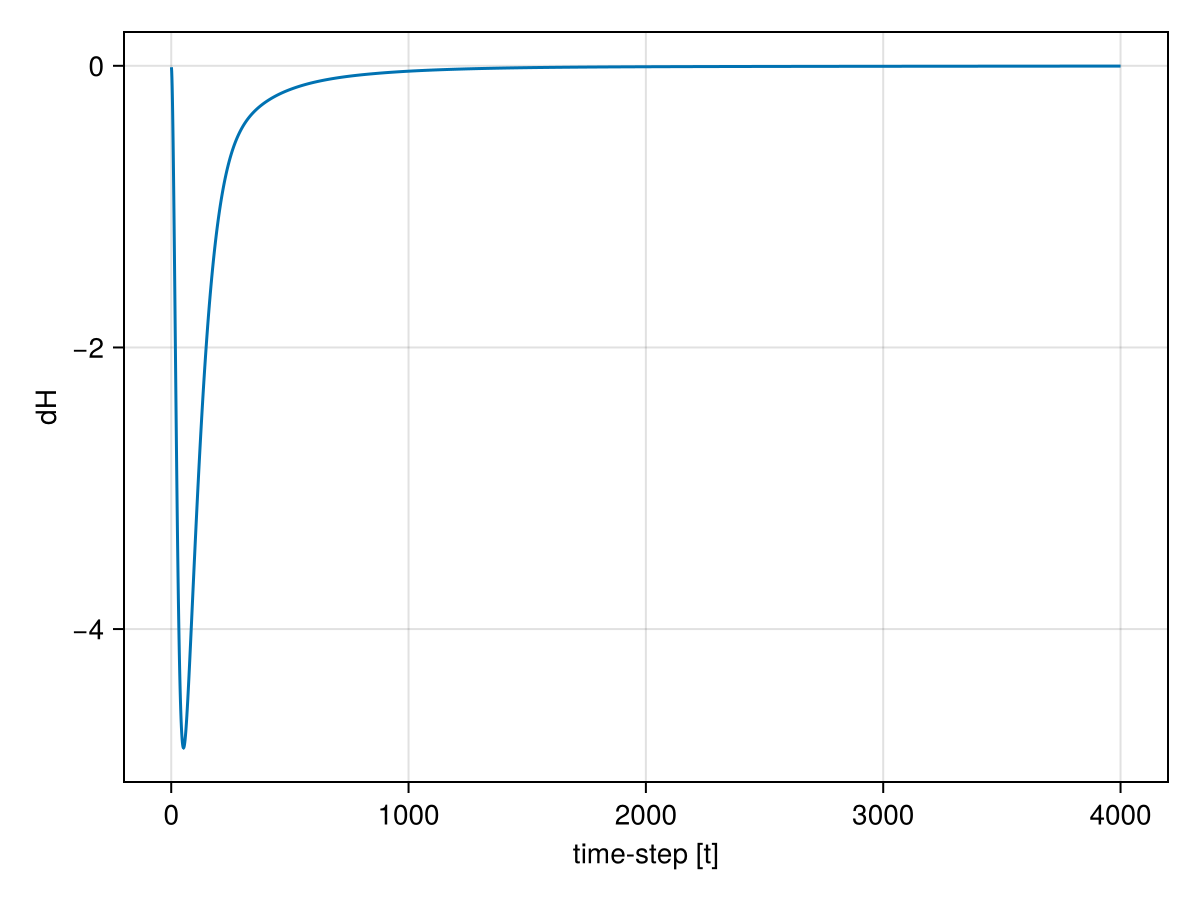
\includegraphics[width=\linewidth]{figures/ch5_basic/dH_crys.png}
        \caption{$\frac{\d}{\d t} H$ over time}
        \label{plot:crys_dh}
    \end{subfigure}
    \caption{Hamiltonian for crystallization with $u_i =0$ with dissipation}
    \label{plot:crys_hamiltonian}
\end{figure}

The Hamiltonian, which is a representation of the total energy of the system relaxes towards lower energy levels, as the system only loses energy without any gain. Simultaneously, the derivative of the Hamiltonian $\frac{\d}{\d t} H$ reaches 0 as the Hamiltonian becomes constant.
\pagebreak

\item \textbf{No dissipation ($\lambda = 0$)}
\begin{figure}[H]
    \centering
    \begin{subfigure}{.49\textwidth}
        \centering
        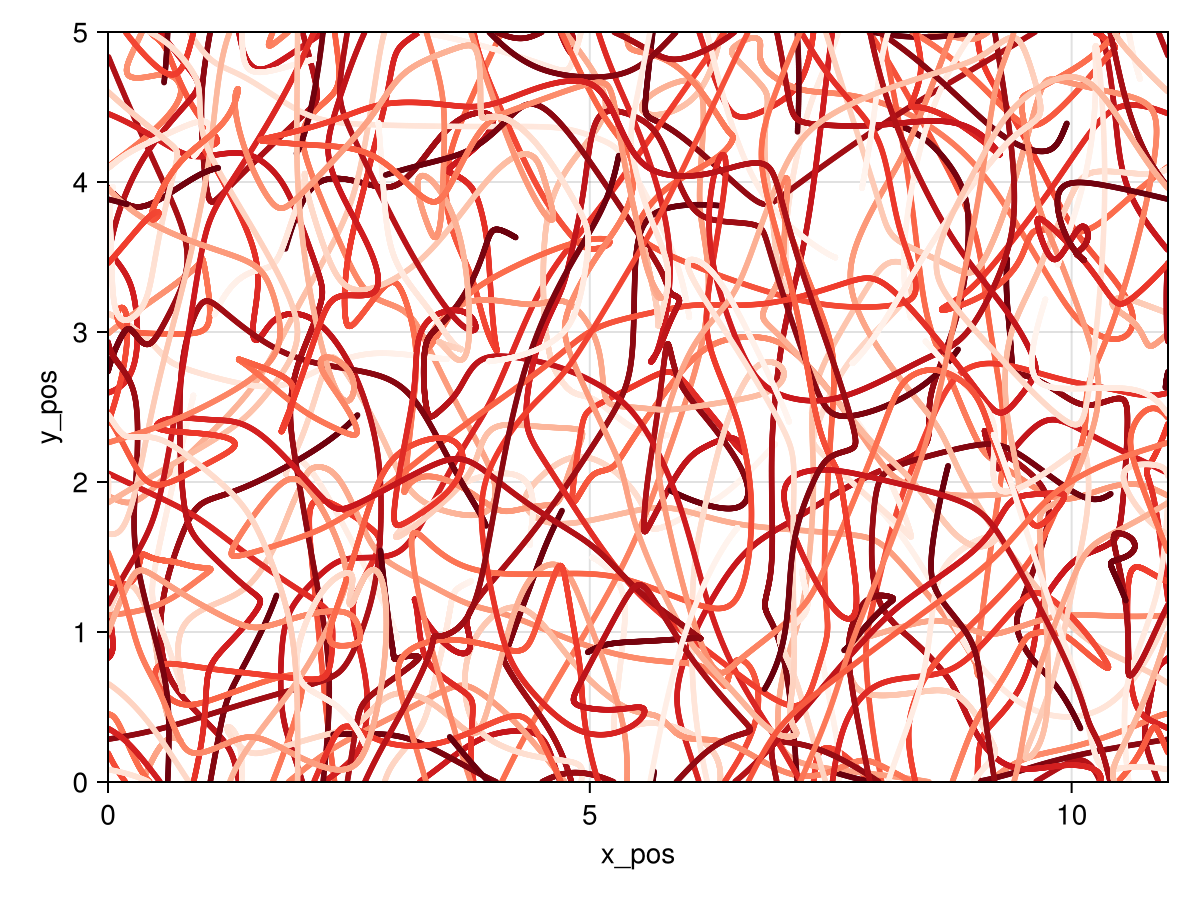
\includegraphics[width=\linewidth]{figures/ch5_basic/traj_nodisp_4000.png}
        \caption{Pedestrian trajectories}
        \label{plot:nodisp_traj}
    \end{subfigure}
    \begin{subfigure}{.49\textwidth}
        \centering
        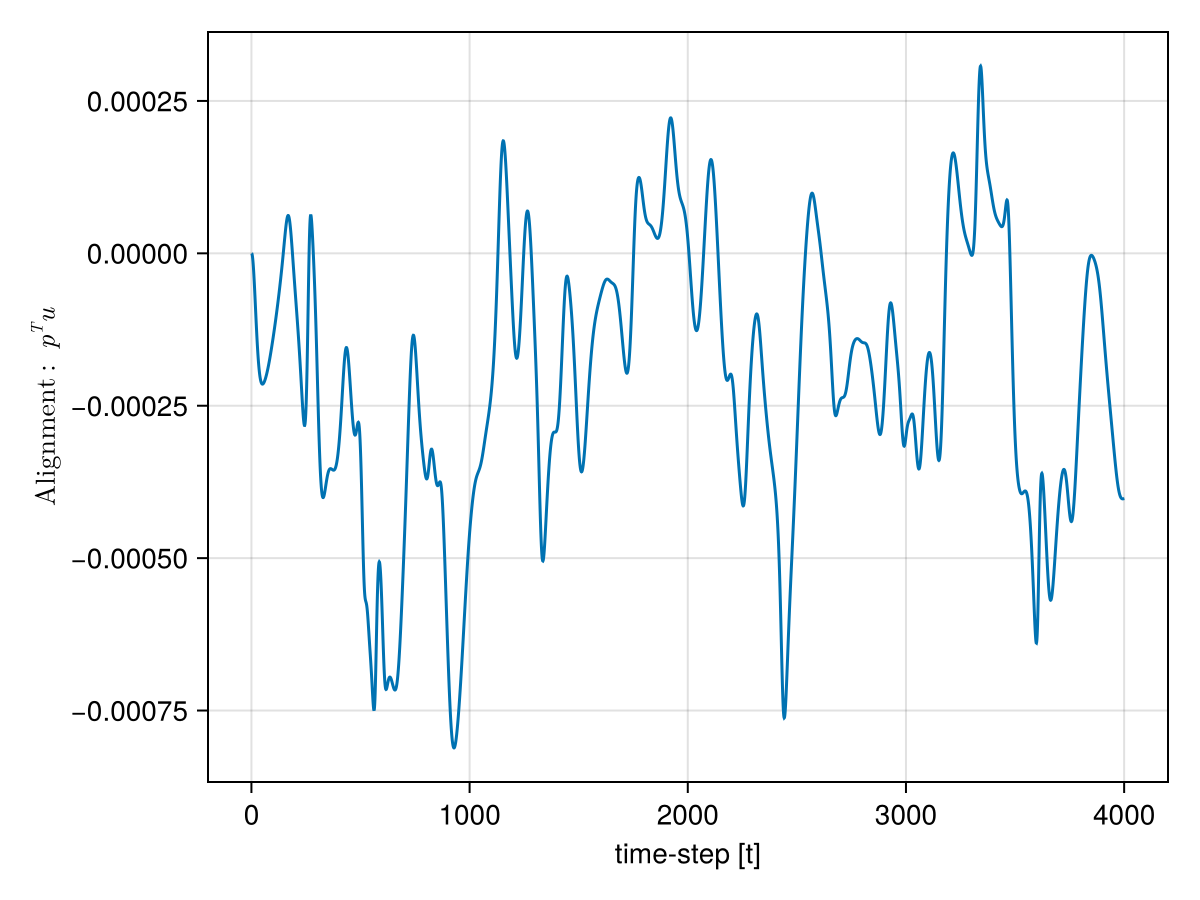
\includegraphics[width=\linewidth]{figures/ch5_basic/straight_nodisp.png}
        \caption{Alignment}
        \label{plot:nodisp_alignment}
    \end{subfigure}
    \caption{Trajectories of pedestrians in a non-dissipative system ($\lambda = 0$)}
    \label{plot:nodisp}
\end{figure}

Given the dynamics formulated in \autoref{eq:ph_model}, it can be clearly seen that $\lambda$ exists both as a coefficient of the input port $\tilde u$ as well as in the output port $y$. Thus setting $\lambda = 0$ clearly suggests that the resulting system has no dissipation as well as no energy feed. Consequently, the pedestrians move with no direction \autoref{plot:nodisp_traj} regardless of the fact that the desired velocity is provided. The disordered directions of all agents is clearly quantified by the alignment measure as the values remain near 0, suggesting the mean direction of all pedestrians is not at all aligned to their desired velocity directions.

\begin{figure}[H]
    \centering
    \begin{subfigure}{0.49\textwidth}
        \centering
        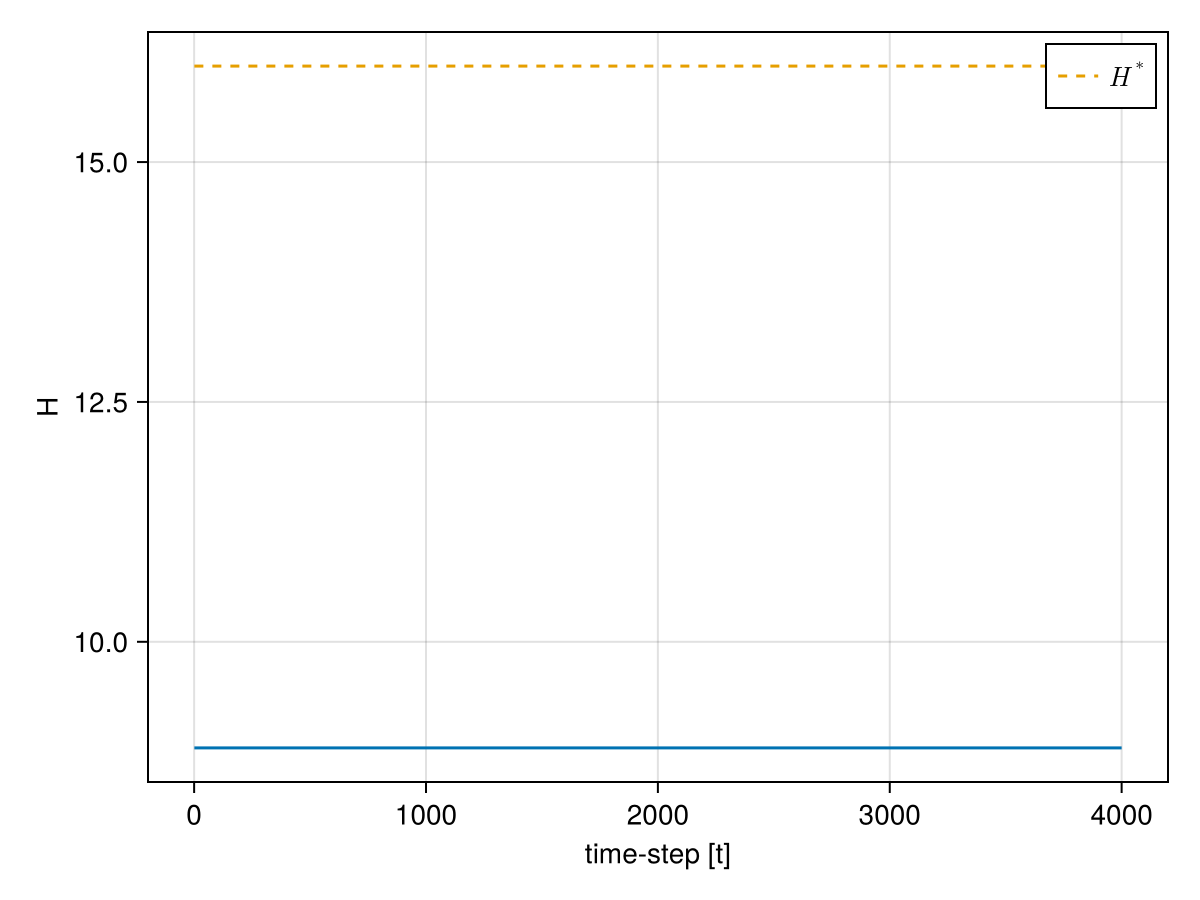
\includegraphics[width=\linewidth]{figures/ch5_basic/H_nodisp.png}
        \caption{Hamiltonian $H$ over time}
        \label{plot:nodisp_h}
    \end{subfigure}
    \begin{subfigure}{.49\textwidth}
        \centering
        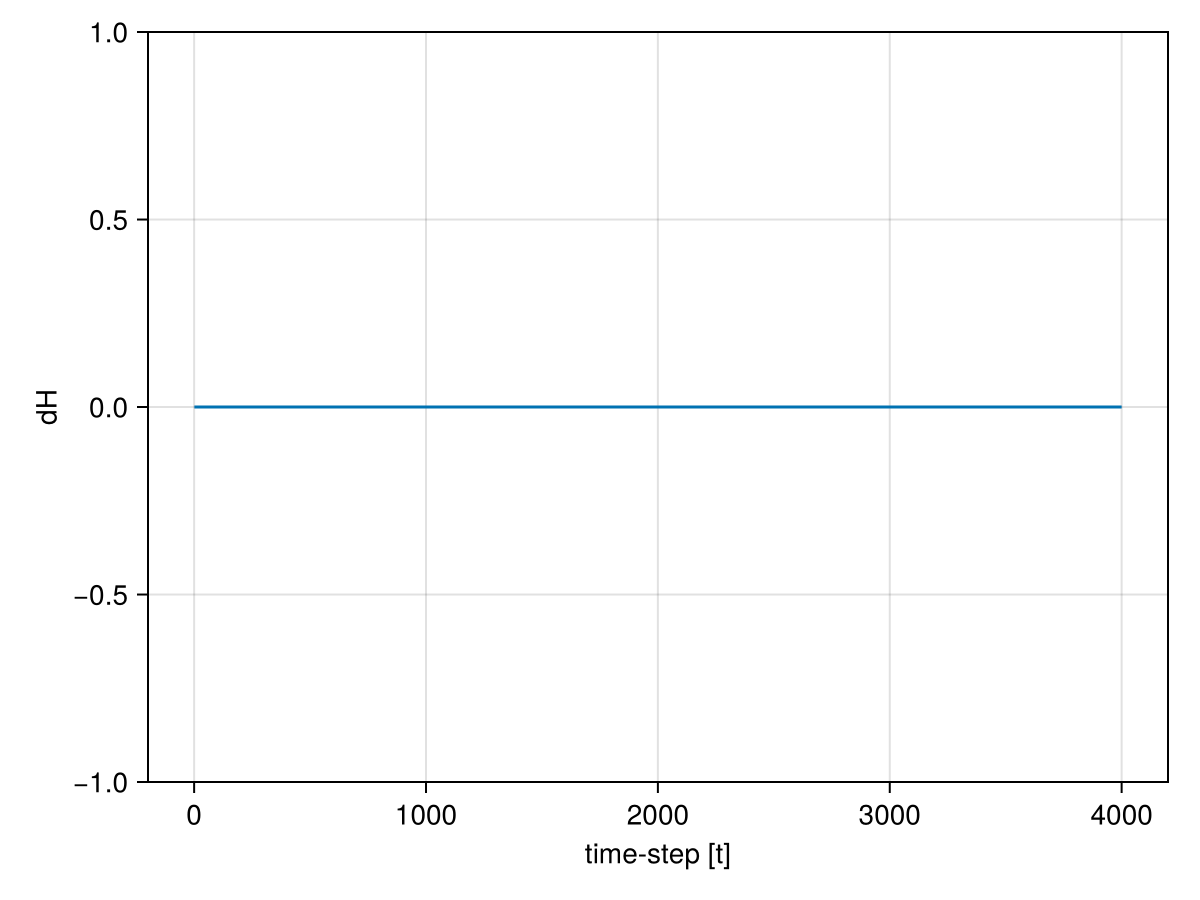
\includegraphics[width=\linewidth]{figures/ch5_basic/dH_nodisp.png}
        \caption{$\frac{\d}{\d t} H$ over time}
        \label{plot:nodisp_dh}
    \end{subfigure}
    \caption{Hamiltonian for crystallization with $u_i =0$ with dissipation}
    \label{plot:nodisp_hamiltonian}
\end{figure}

The resulting system is a conservative Hamiltonian system \autoref{eq:conservative}, as by consequence the dissipative term $R$ also vanishes. This can be clearly observed as the Hamiltonian remains constant over time.

\item \textbf{No pedestrian interaction ($A = 0$) with $u_i = \begin{bmatrix} 1 & 0 \end{bmatrix}$}
\begin{figure}[H]
    \centering
    \begin{subfigure}{.49\textwidth}
        \centering
        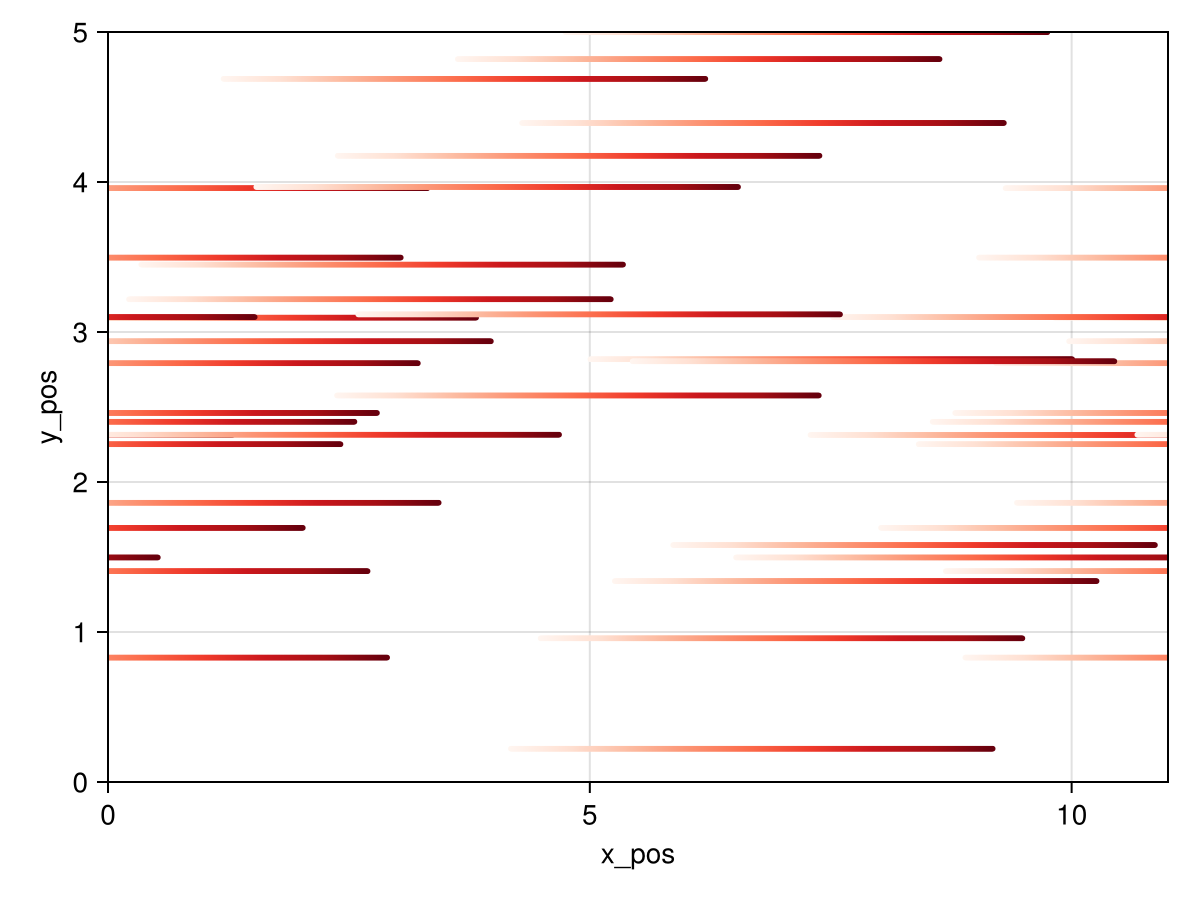
\includegraphics[width=\linewidth]{figures/ch5_basic/traj_nointeraction_4000.png}
        \caption{Pedestrian trajectories}
        \label{plot:nointeraction_traj}
    \end{subfigure}
    \begin{subfigure}{.49\textwidth}
        \centering
        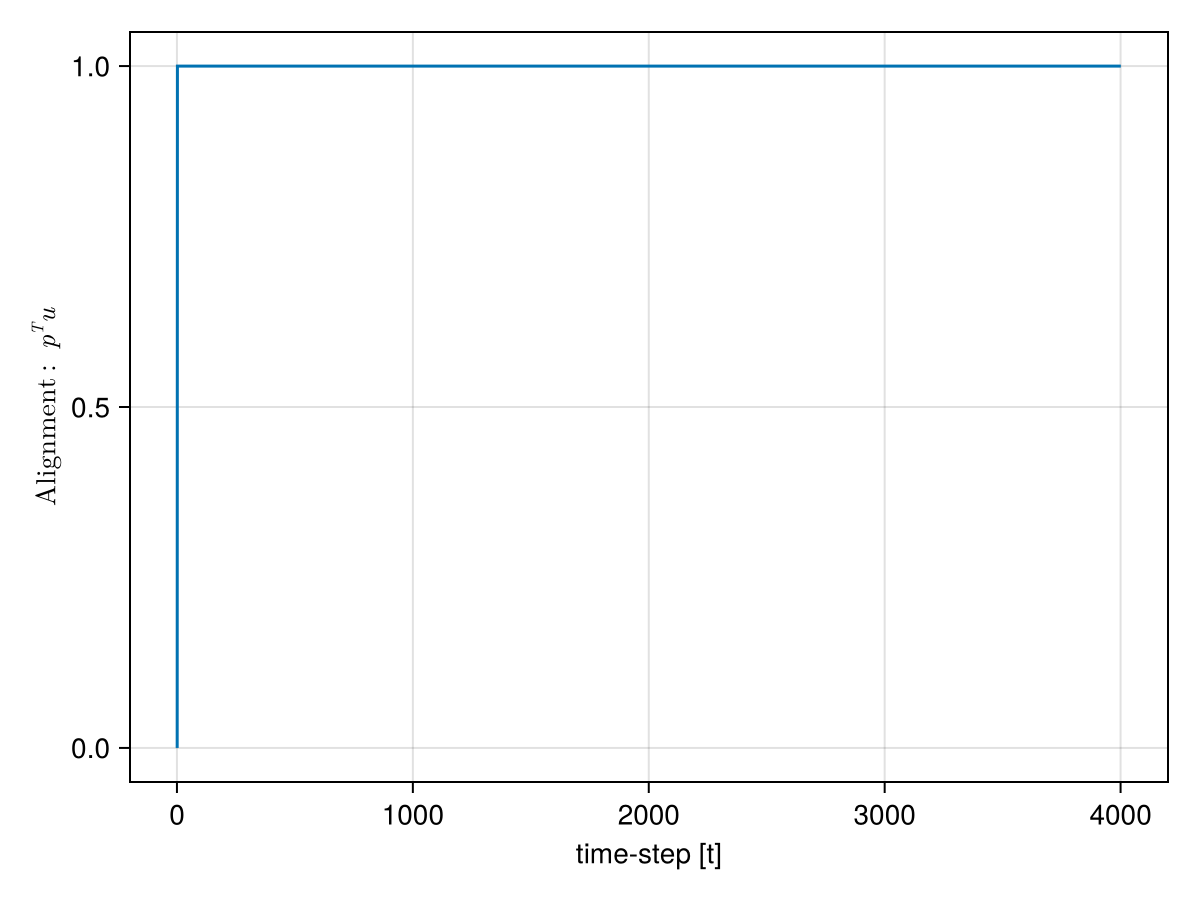
\includegraphics[width=\linewidth]{figures/ch5_basic/straight_nointeraction.png}
        \caption{Alignment}
        \label{plot:nointeraction_alignemnt}
    \end{subfigure}
    \caption{Trajectories of pedestrians with no interaction with other pedestrian ($ A = 0 $) and desired velocities $u_i = \begin{bmatrix}1 & 0\end{bmatrix} $}
    \label{plot:nointeraction}
\end{figure}

By setting $A = 0$, the pedestrians in the system move with no interactivity with other pedestrians in the system. Essentially, every pedestrian simply moves with their desired velocities as soon as the simulation begins \autoref{plot:nointeraction}. Because this parameter directly effects the interaction potential $U(x)$ in \autoref{eq:def_potU}, it can be clearly observed that the motion of the pedestrian is independent of their distance to each other, in other words they move with no concern to how close or far they are from other pedestrians. The alignment plot clearly quantifies this behavior as the plot linearly jumps from 0 to 1, indicating that that all pedestrians accelerate toward their desired directions without disruptions as soon as the simulation begins.


\begin{figure}[H]
    \centering
    \begin{subfigure}{.49\textwidth}
        \centering
        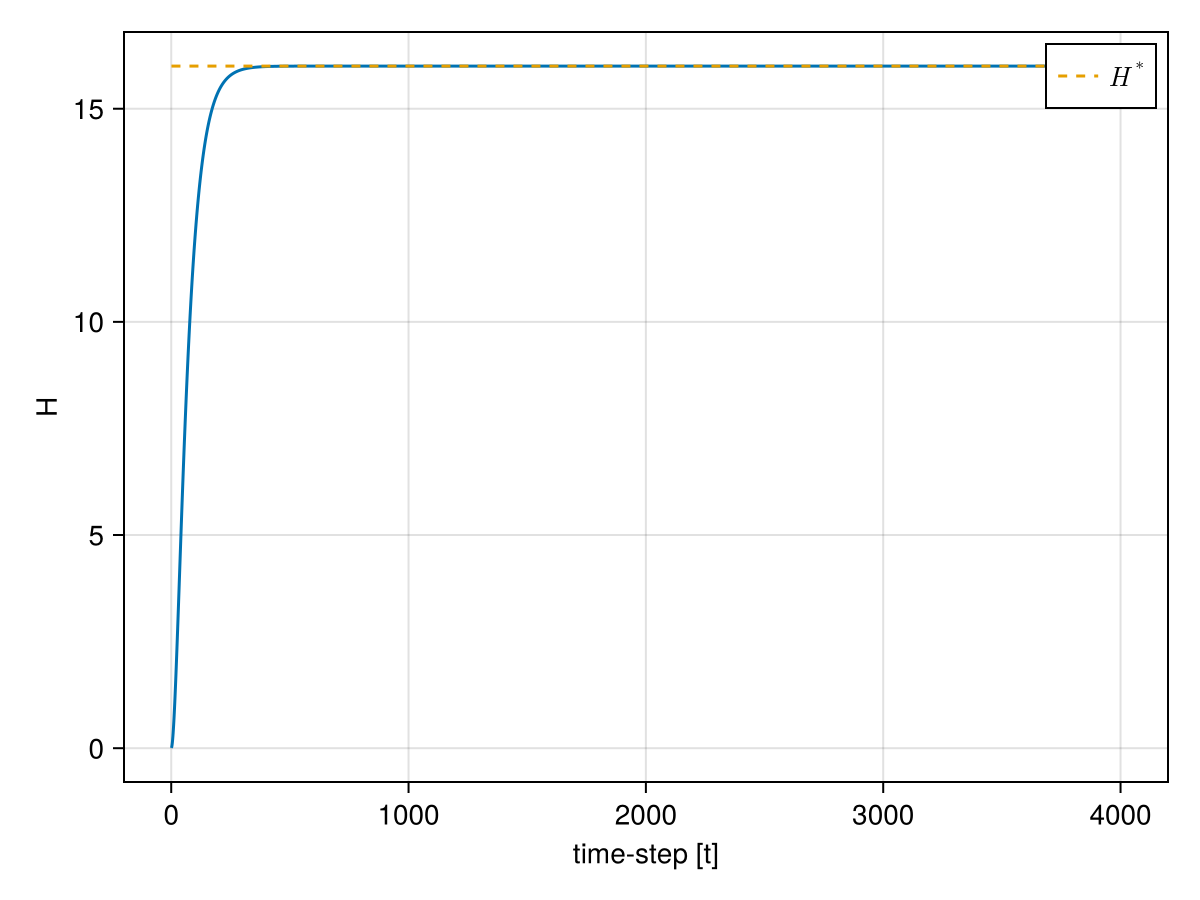
\includegraphics[width=\linewidth]{figures/ch5_basic/H_nointeraction.png}
        \caption{Hamiltonian $H$ over time}
        \label{plot:nointeraction_h}
    \end{subfigure}
    \begin{subfigure}{.49\textwidth}
        \centering
        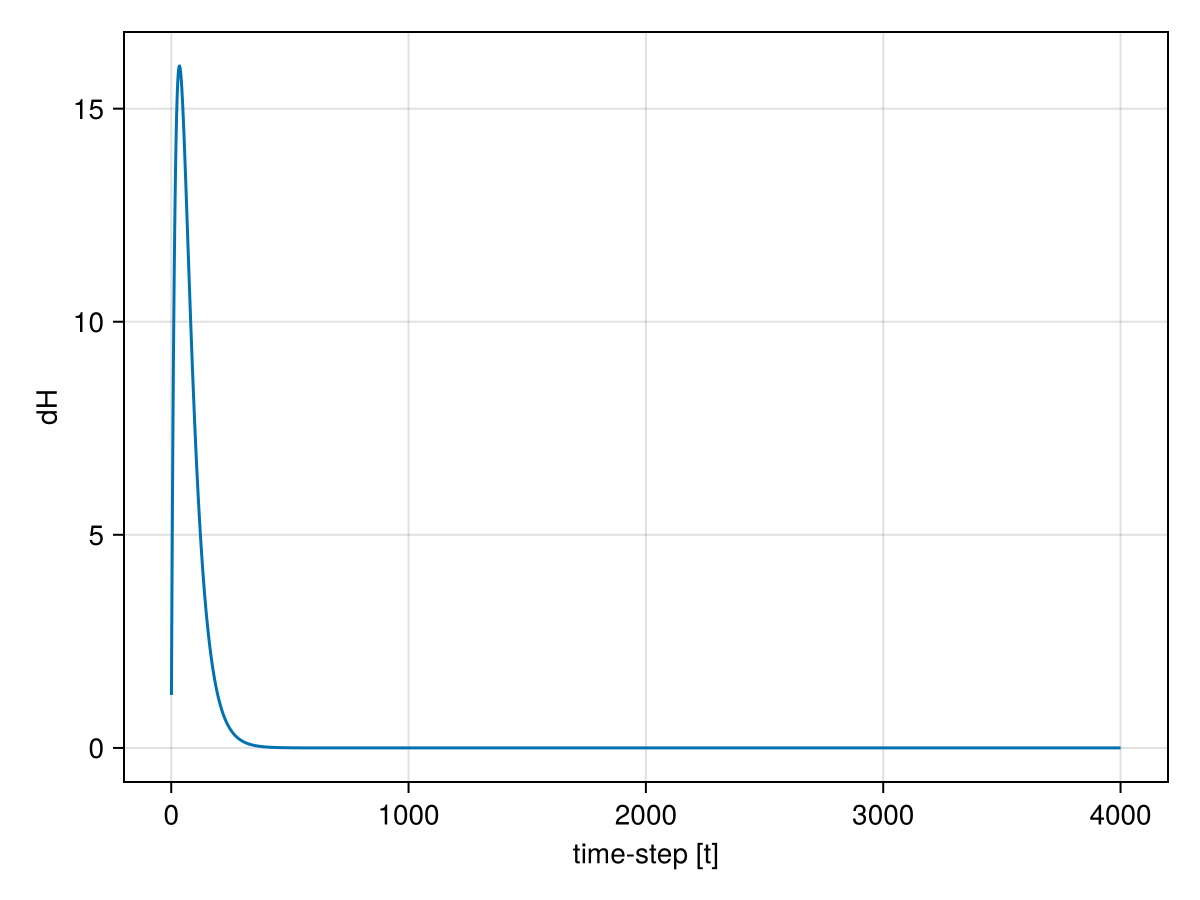
\includegraphics[width=\linewidth]{figures/ch5_basic/dH_nointeraction.png}
        \caption{$\frac{\d}{\d t} H$ over time}
        \label{plot:nointeraction_dh}
    \end{subfigure}
    \caption{Hamiltonian over time with no interaction ($ A = 0 $) and desired velocities $u_i = \begin{bmatrix}1 & 0\end{bmatrix} $}
    \label{plot:nointeraction_hamiltonian}
\end{figure}

Given the lack of interaction, the pedestrians move with their desired velocities, thus the Hamiltonian need not be dependent on time, but instead on the desired velocities of the pedestrians -- mathematically $p_i = u_i$. One can also obtain this long term value of the Hamiltonian $H^*(u)$ by setting $A = 0$ (as it is for this case) in \autoref{eq:Hamiltonian} leading to 
\begin{align}
    H(z(t)) = \dfrac{1}{2}||p(t)||^2 \rightarrow H^*(u) = \dfrac{1}{2}||u||^2
    \label{eq:Hstar}
\end{align}

This expression for the long term Hamiltonian $H^*(u)$ is a function of the desired velocities $u_i$. As $u_i$ is set by the user, one easily evaluate this value. Even with potential interaction allowed in the system dynamics, the expression serves as a representation of what the system as a whole is trying to attain. Ideally, every pedestrian wants to achieve the desired velocity $u_i$, and the system as a whole wants to achieve the energy $H^*$. 
\end{itemize}

\subsection{Collective Dynamics}
\label{section:collective}

In this section, we will witness collective phenomenon based on the desired speeds and relaxation (or dissipation) parameter $\lambda$. The pedestrians will start from the same random positions generated in \autoref{plot:starting_pos}, but with different desired speeds $u_i$. This disordered arrangement goes through a phase transition and form ordered patterns, such as lane formation and stripe formation. We will notice how a sufficient $\lambda$ is needed to achieve these phase transitions. Furthermore, we will see how $H^*(u)$ from \autoref{eq:Hstar} ties in as an order parameter to identify collective behaviors.
\begin{itemize}
    \item \textbf{Lane Formation for counter flow with $\lambda = 2$}
    \begin{figure}[H]
        \centering
        \begin{subfigure}{.49\textwidth}
            \centering
            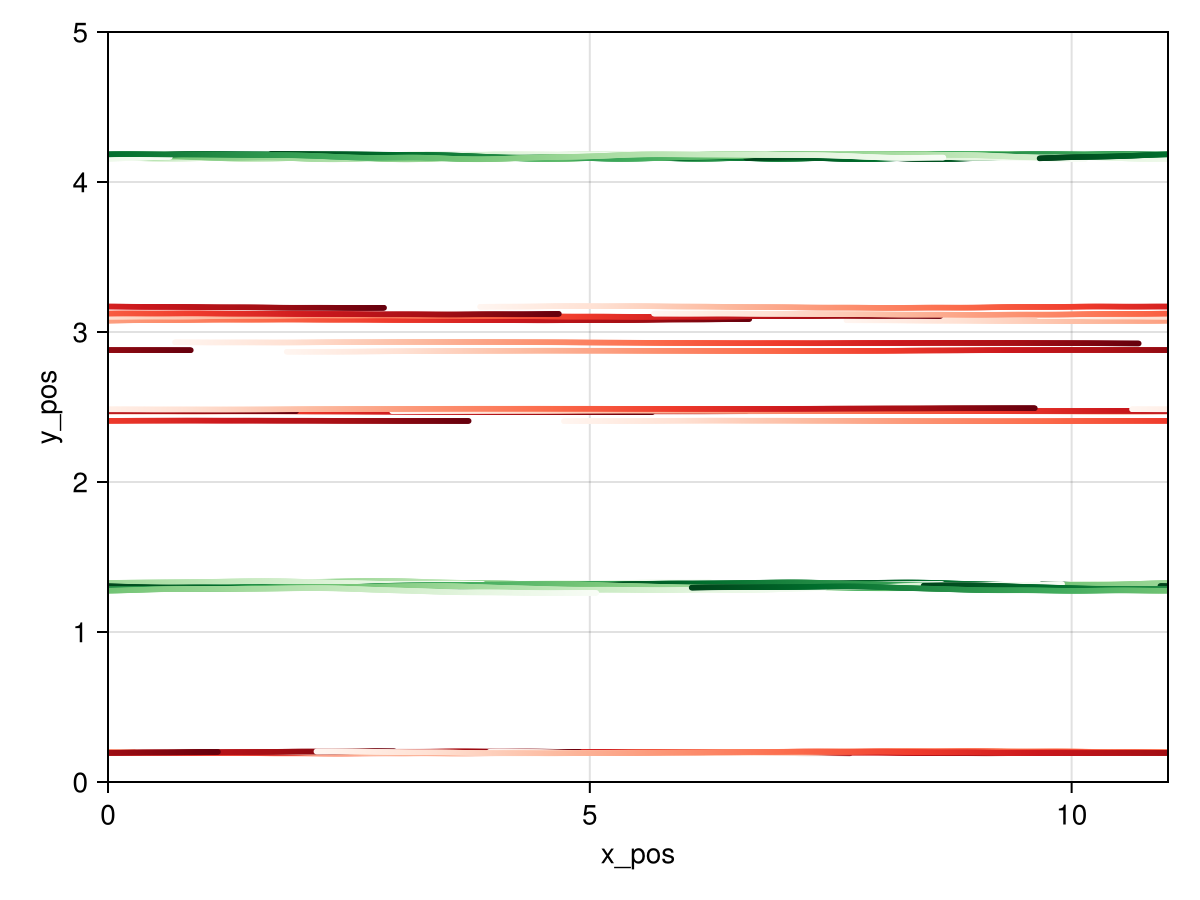
\includegraphics[width=\linewidth]{figures/ch5_collective/counter.png}
            \caption{Pedestrian trajectories}
            \label{plot:counter_traj}
        \end{subfigure}
        \begin{subfigure}{.49\textwidth}
            \centering
            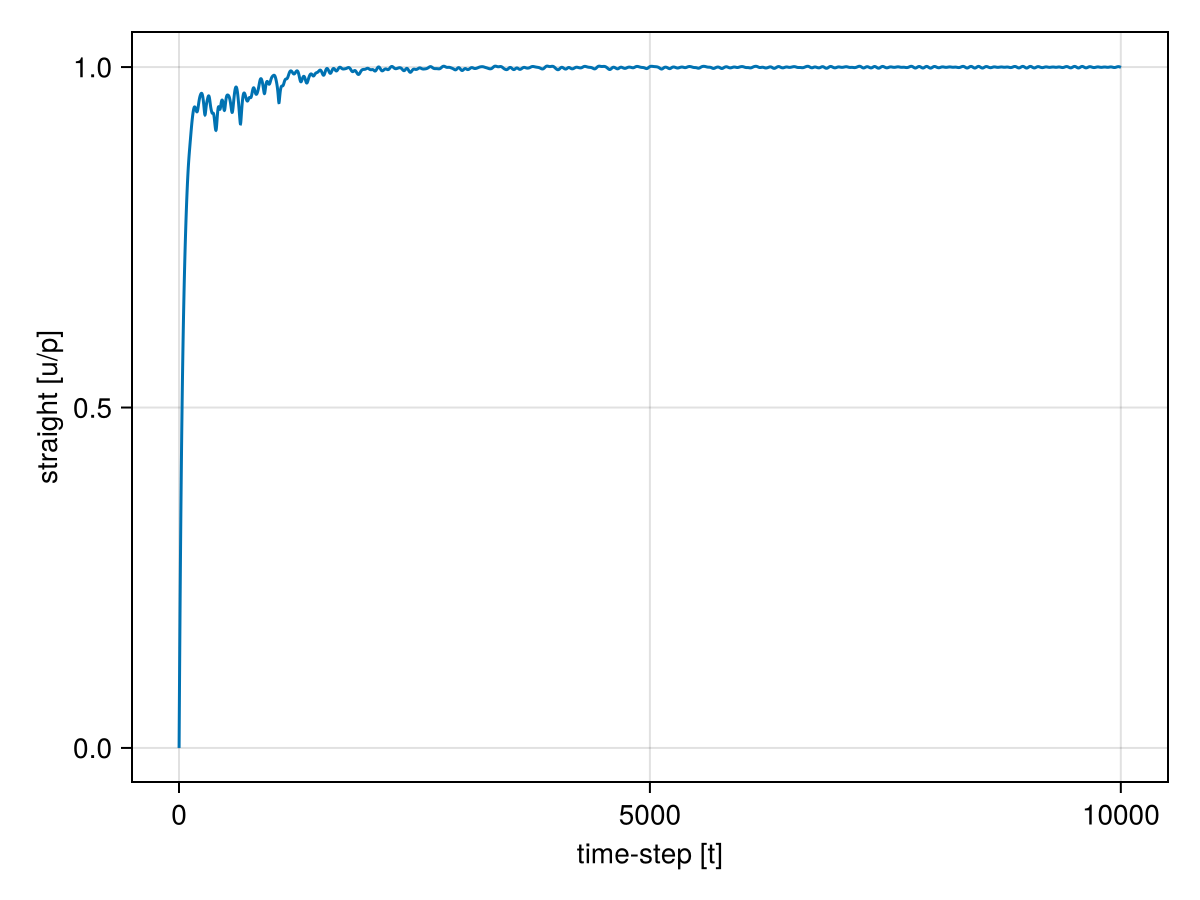
\includegraphics[width=\linewidth]{figures/ch5_collective/straight_counter.png}
            \caption{Alignment}
            \label{plot:counter_alignment}
        \end{subfigure}
        \caption{Lane formation for counter flow}
        \label{plot:counter}
    \end{figure}
Starting from a random arrangement of pedestrians as shown in \autoref{plot:starting_pos}, with predefined desired velocities $u_i = \begin{bmatrix} 1 & 0 \end{bmatrix}$ for half of the pedestrians (Red), and $u_i = \begin{bmatrix} -1 & 0 \end{bmatrix}$ for the other half (Green), as shown in \autoref{code:agent_init}. As the time progresses, the pedestrians form lanes. The alignment clearly illustrates transition from disorder to order, as the pedestrians align themselves to their respective desired velocities over time.
    \begin{figure}[H]
        \centering
        \begin{subfigure}{.49\textwidth}
            \centering
            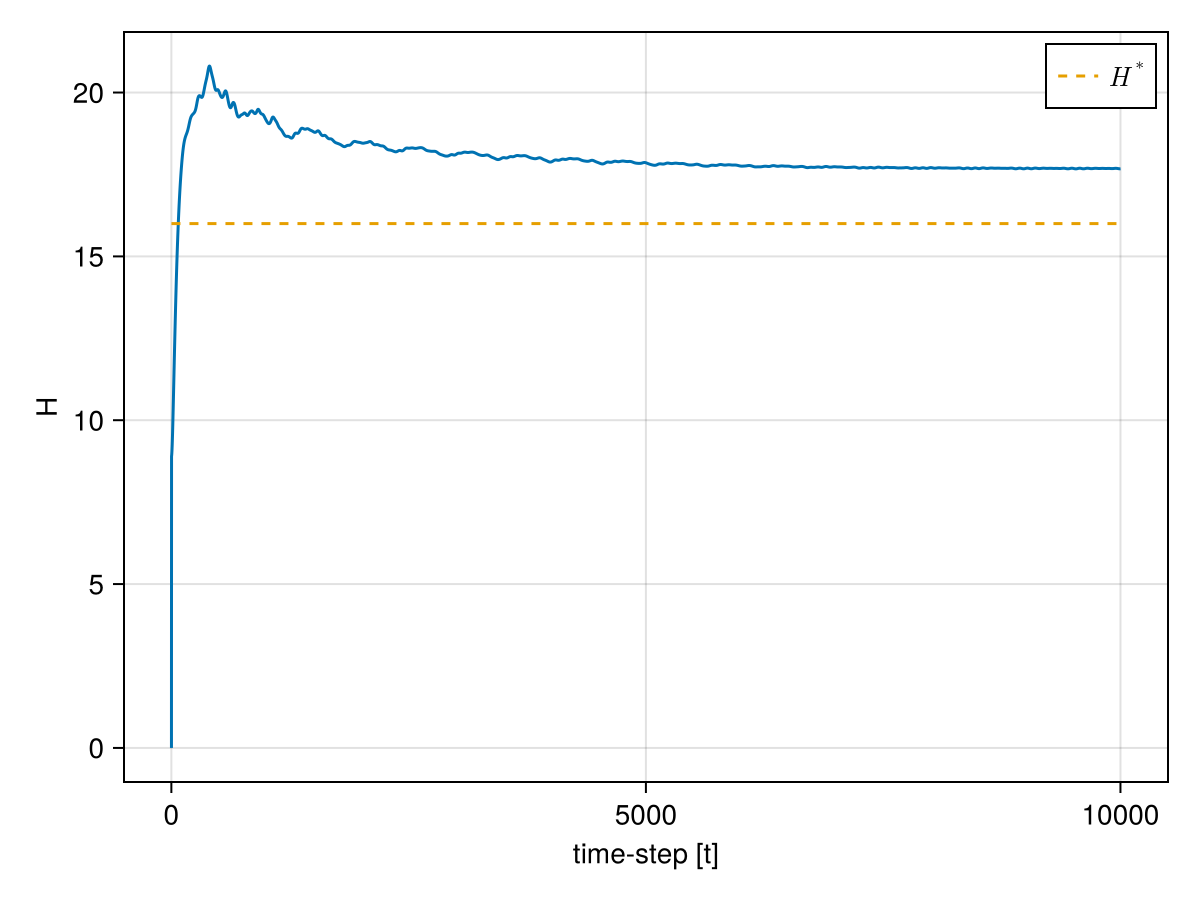
\includegraphics[width=\linewidth]{figures/ch5_collective/H_counter.png}
            \caption{Hamiltonian $H$ over time}
            \label{plot:counter_h}
        \end{subfigure}
        \begin{subfigure}{.49\textwidth}
            \centering
            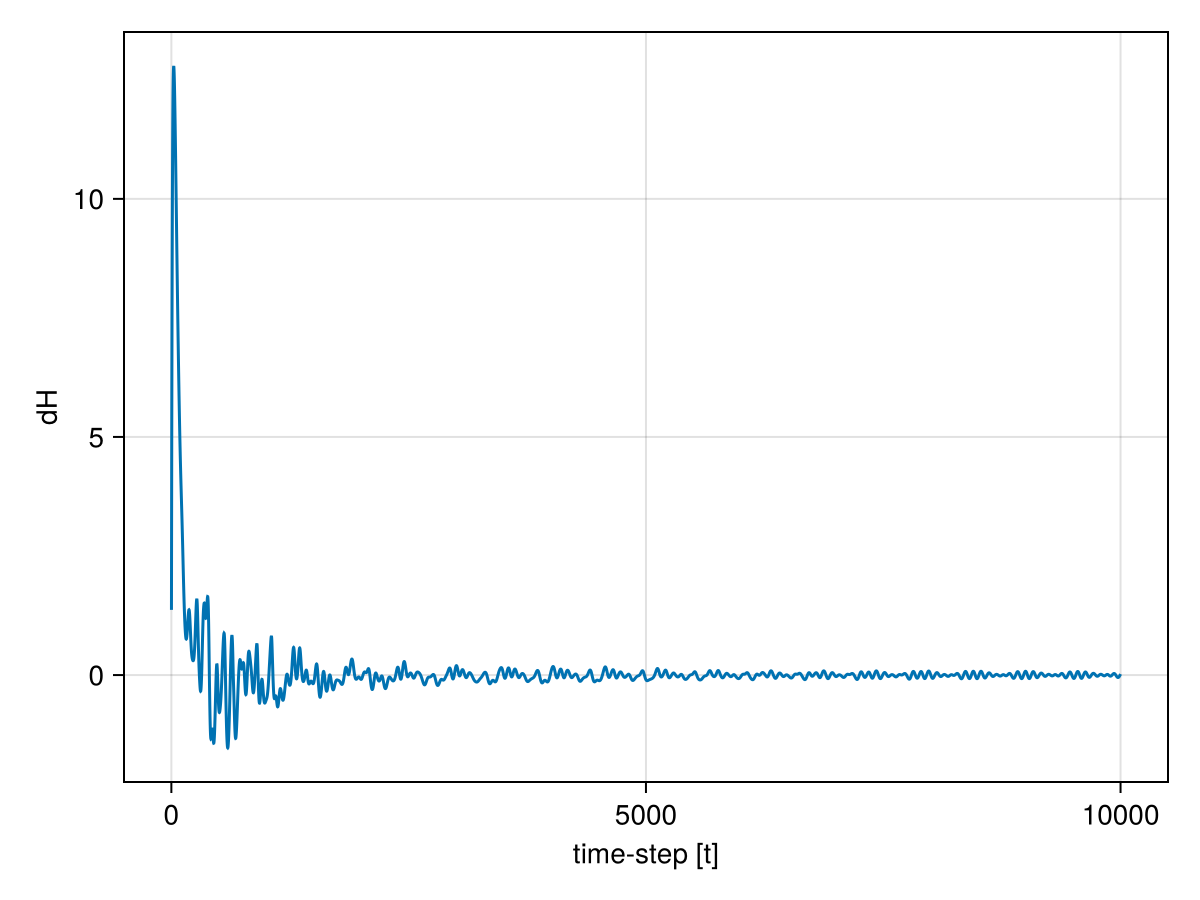
\includegraphics[width=\linewidth]{figures/ch5_collective/dH_counter.png}
            \caption{$\frac{d}{dt}H$ over time}
            \label{plot:counter_dh}
        \end{subfigure}
        \caption{Hamiltonian for counter flow with lane formation}
        \label{plot:counter_hamiltonian}
    \end{figure}
From the point of view of energy in the system, the pedestrians self-organize themselves in a manner such that the Hamiltonian reaches a steady state and remains above $H^*$, while $\frac{d}{dt}H$ converges to zero. 

    \item \textbf{Gridlock for counter flow with $\lambda = 0.2$}
    \begin{figure}[H]
        \centering
        \begin{subfigure}{0.49\textwidth}
            \centering
            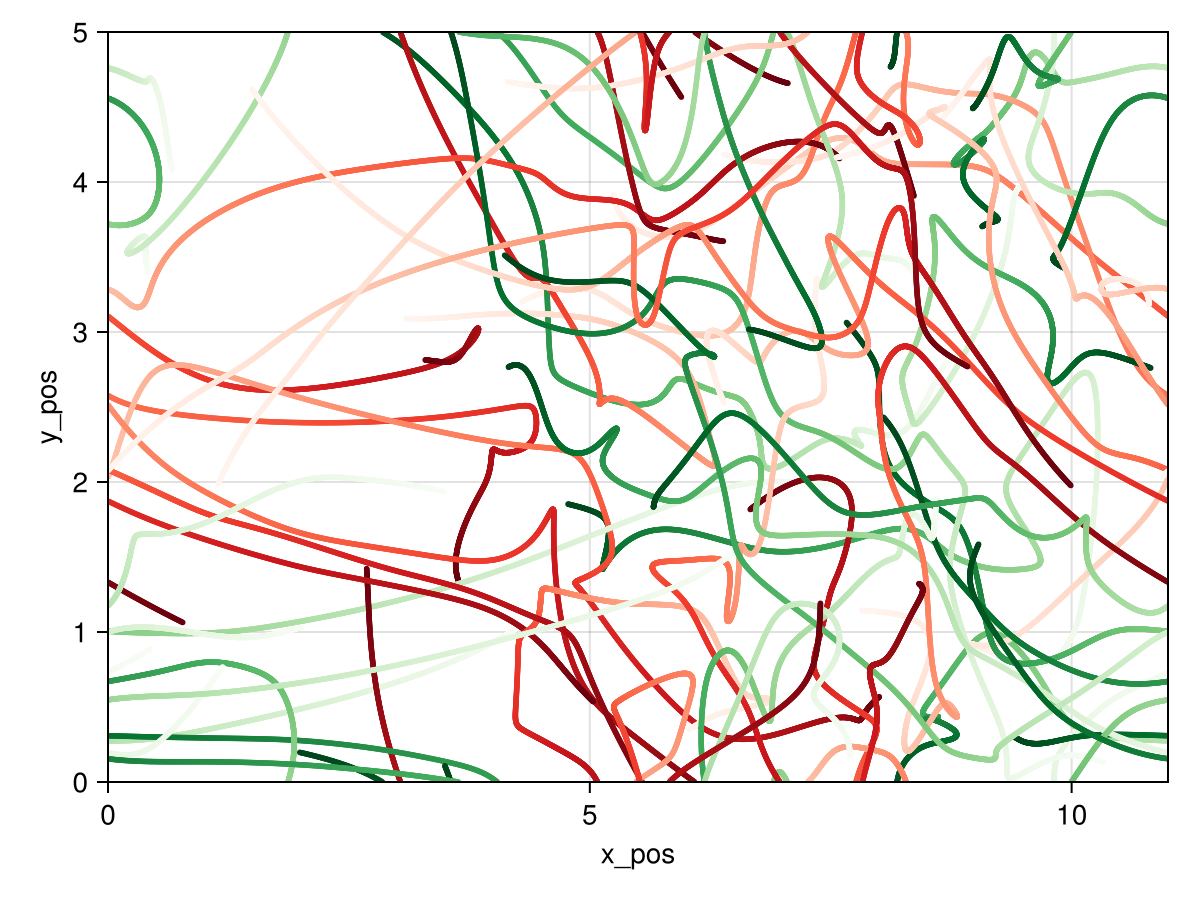
\includegraphics[width=\linewidth]{figures/ch5_collective/counter_gridlockdflow_4000.png}
            \caption{Pedestrian trajectories}
            \label{plot:countergridlock_traj}
        \end{subfigure}
        \begin{subfigure}{.49\textwidth}
            \centering
            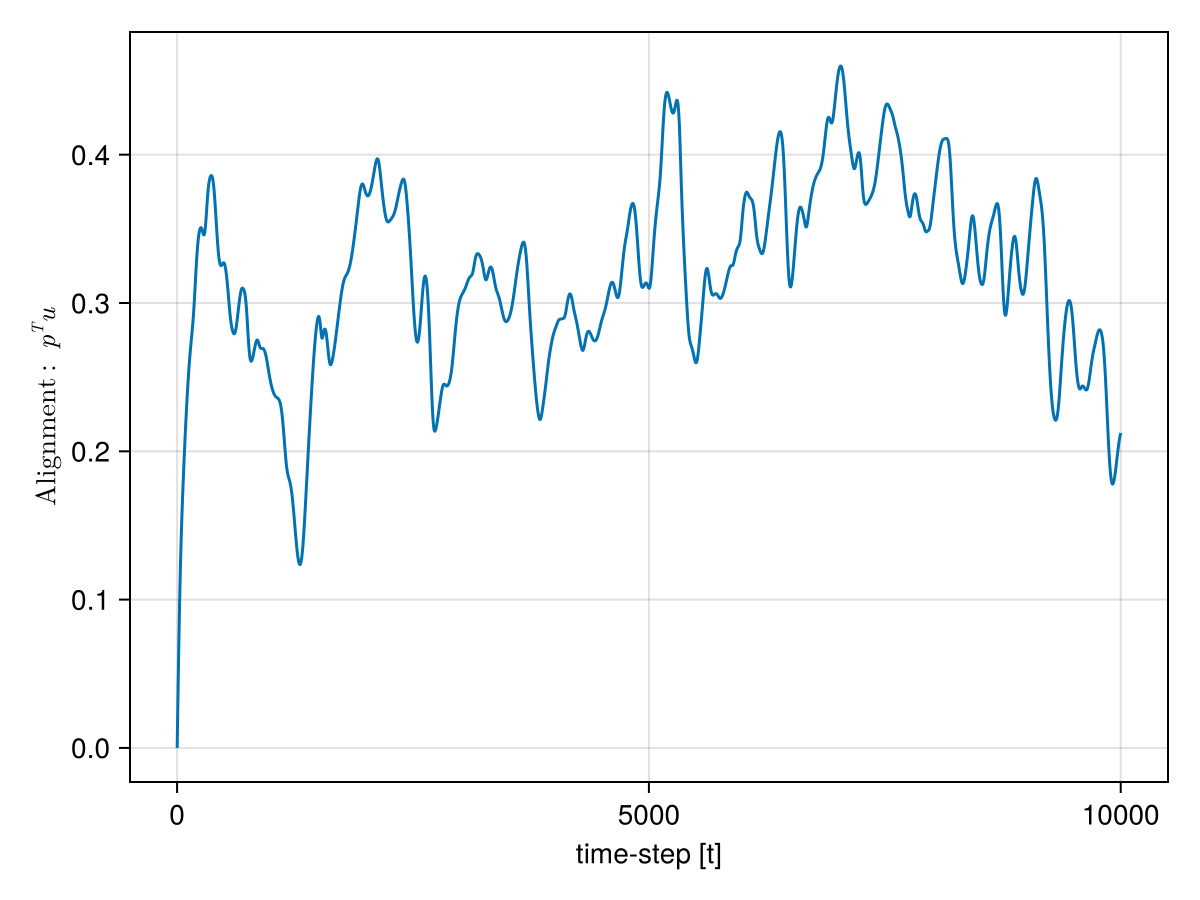
\includegraphics[width=\linewidth]{figures/ch5_collective/straight_gridlock_counter.png}
            \caption{Alignment}
            \label{plot:countergridlock_alignment}
        \end{subfigure}
        \caption{Gridlock for counter flow}
        \label{plot:countergridlock}
    \end{figure}
With the same parameters as the previous case, with the only difference being that $\lambda$ is not sufficiently high, it can be observed that no lane formation occurs. The system neither gains nor dissipates enough energy, resulting in pedestrians behaving similarly to the trajectories presented in \autoref{plot:nodisp}, leading to gridlocks. Since the pedestrians fail to reach their desired directions, the alignment stays near zero indicating disorder in the system, as it can be clearly witnessed from the trajectories.
    \begin{figure}[H]
        \centering
        \begin{subfigure}{.49\textwidth}
            \centering
            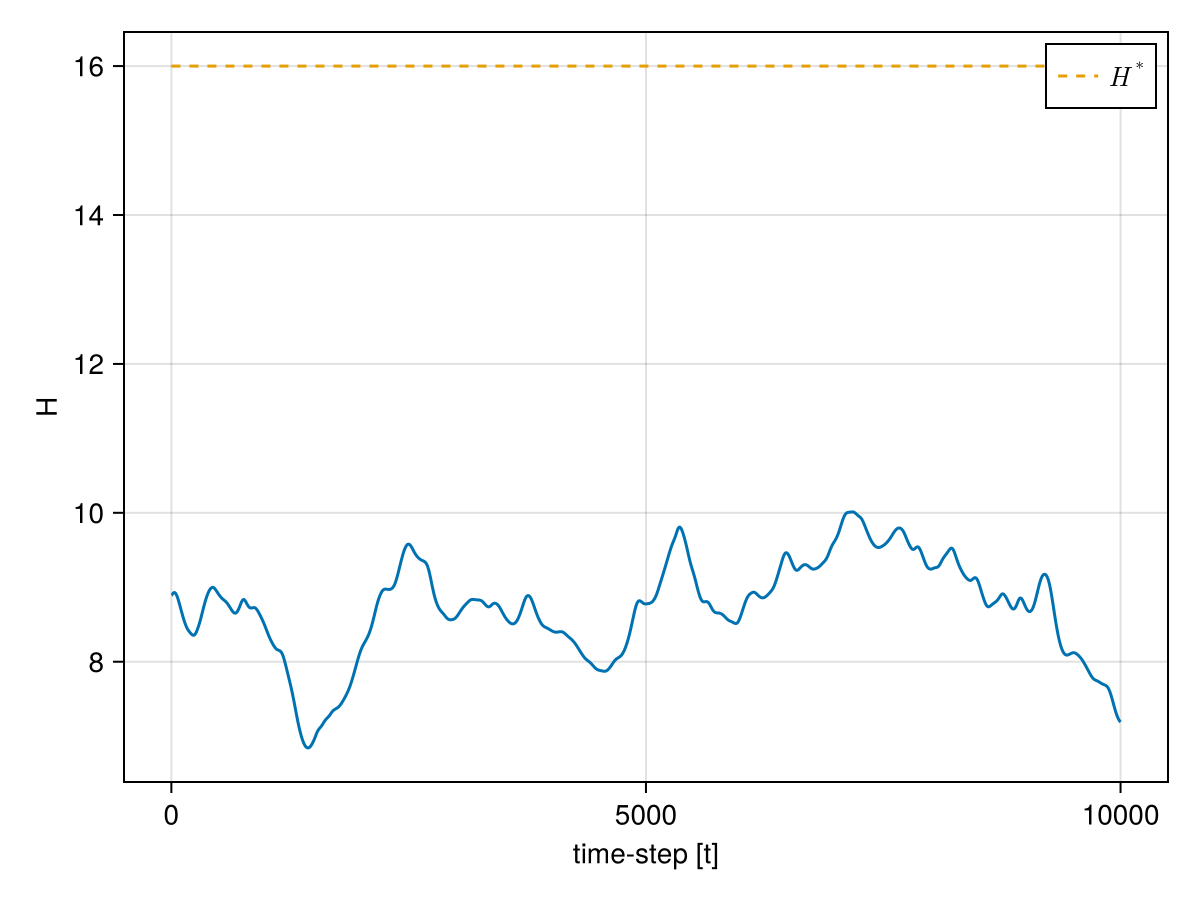
\includegraphics[width=\linewidth]{figures/ch5_collective/H_gridlock_counter.png}
            \caption{Hamiltonian $H$ over time}
            \label{plot:countergridlock_h}
        \end{subfigure}
        \begin{subfigure}{.49\textwidth}
            \centering
            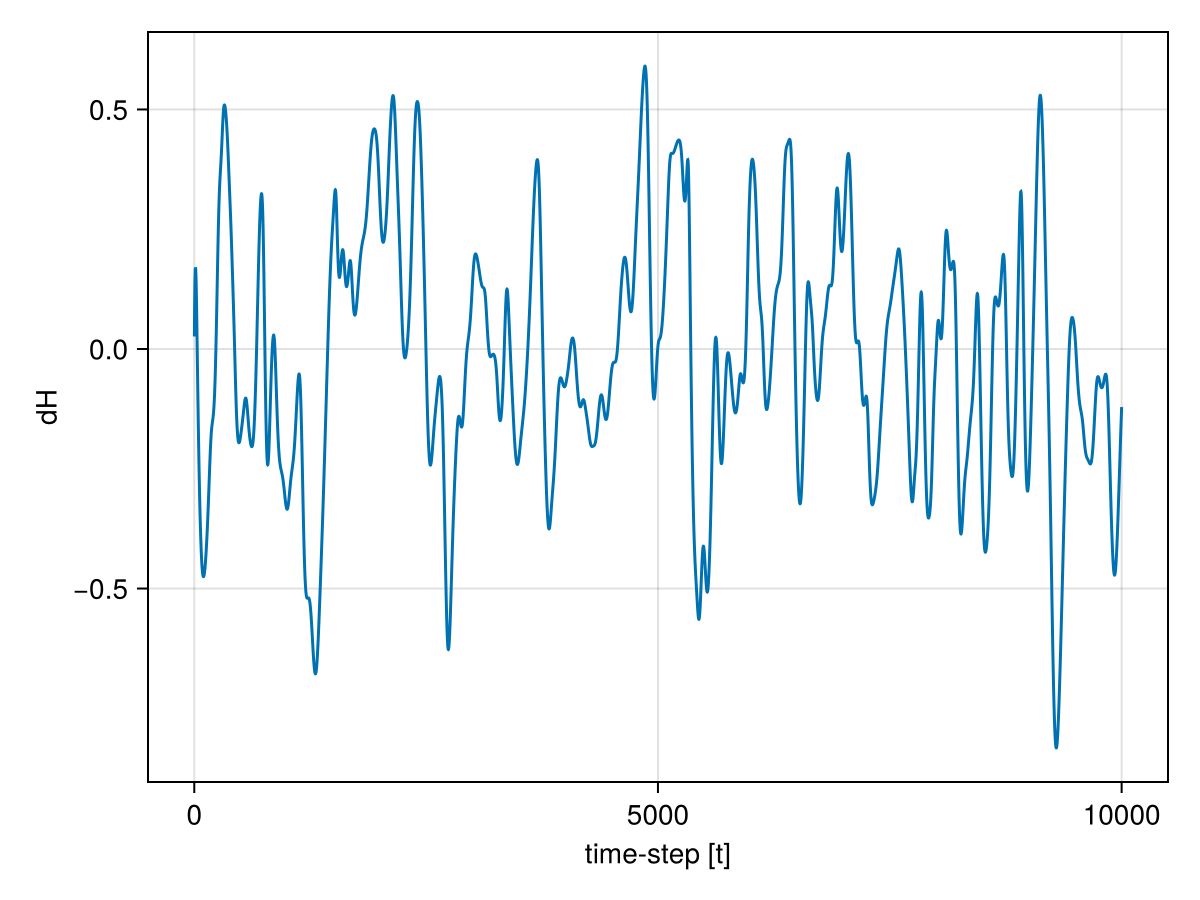
\includegraphics[width=\linewidth]{figures/ch5_collective/dH_gridlock_counter.png}
            \caption{$\frac{d}{dt}H$ over time}
            \label{plot:countergridlock_dh}
        \end{subfigure}
        \caption{Hamiltonian for counter flow with gridlock}
        \label{plot:countergridlock_hamiltonian}
    \end{figure}


The Hamiltonian erratically fluctuates over time and remains below $H^*$. Here the significance of $\lambda$ is apparent, as this parameter balances the conservation of energy enforced by the skew-symmetry with the flow of energy through dissipation and feed permitted by the ports.

    \item \textbf{Stripe Formation for cross flow with $\lambda = 2$}
    \begin{figure}[H]
        \centering
        \begin{subfigure}{0.49\textwidth}
            \centering
            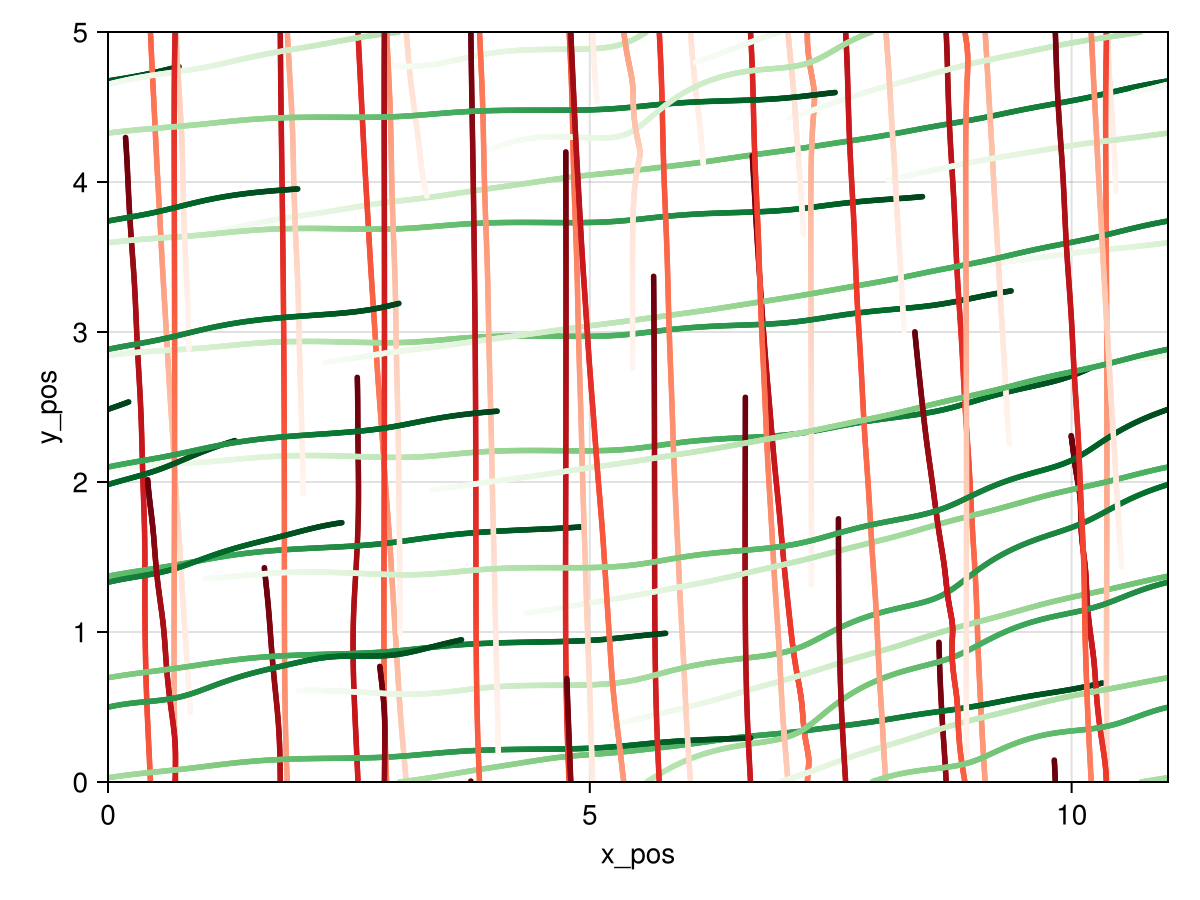
\includegraphics[width=\linewidth]{figures/ch5_collective/crossleapflow_10000.png}
            \caption{Pedestrian trajectories}
            \label{plot:cross2_traj}
        \end{subfigure}
        \begin{subfigure}{.49\textwidth}
            \centering
            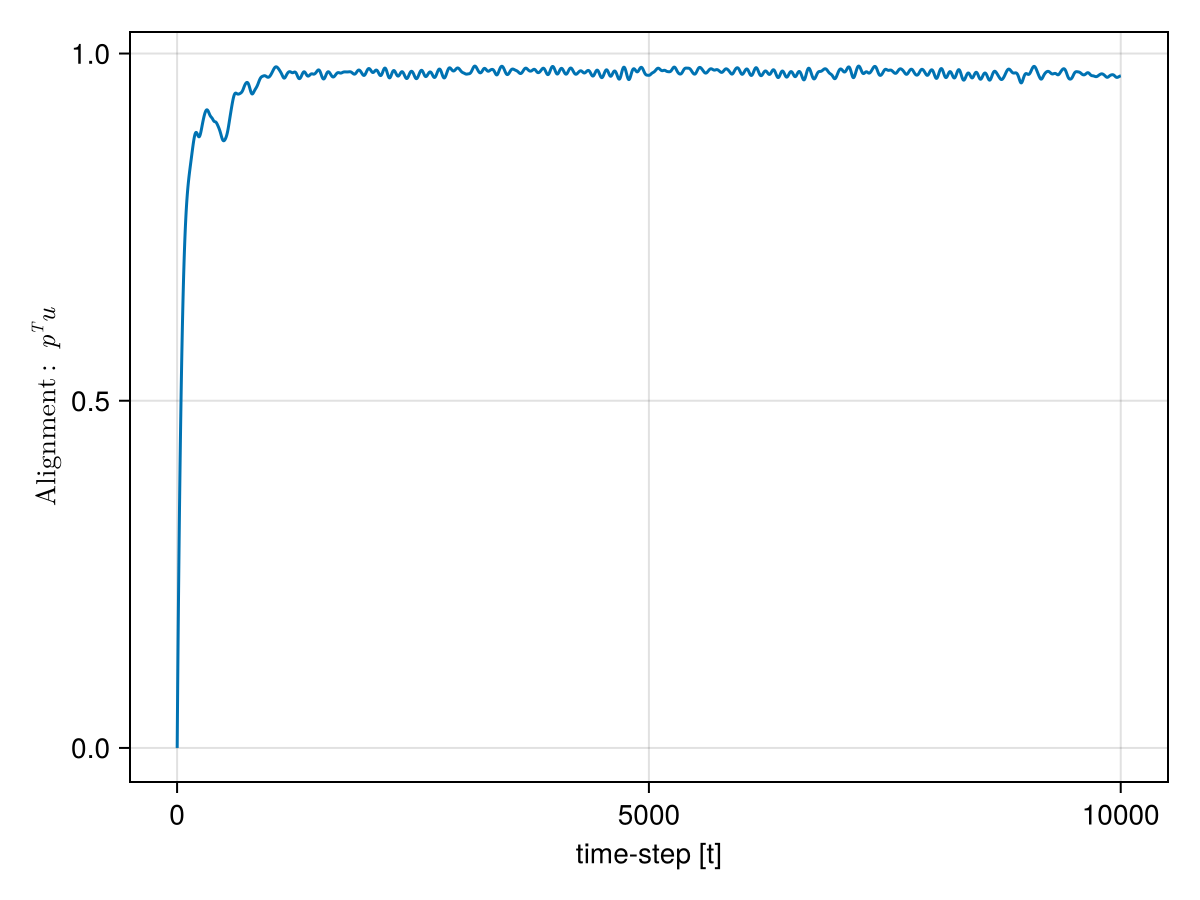
\includegraphics[width=\linewidth]{figures/ch5_collective/straight_cross2.png}
            \caption{Alignment}
            \label{plot:cross2_alignment}
        \end{subfigure}
        \caption{Stripe formation at a diagonal for cross flow with $\lambda = 2$}
        \label{plot:cross2}
    \end{figure}
Starting from the same positions as \autoref{plot:starting_pos} with the desired velocities set to $u_i = \begin{bmatrix} 1 & 0 \end{bmatrix}$ for half of the pedestrians (Green), and $u_i = \begin{bmatrix} 0 & 1 \end{bmatrix}$ for the other half (Red). We can observe that the pedestrians form a \textit{diagonal} stripe formation; they are not able to reach the desired direction with much ease, forming angled stripes. Interestingly, alignment remains near but below 1, clearly indicating that the pedestrians are not quite able to reach their desired velocities even though the overall system is still ordered.

    \begin{figure}[H]
        \centering
        \begin{subfigure}{.49\textwidth}
            \centering
            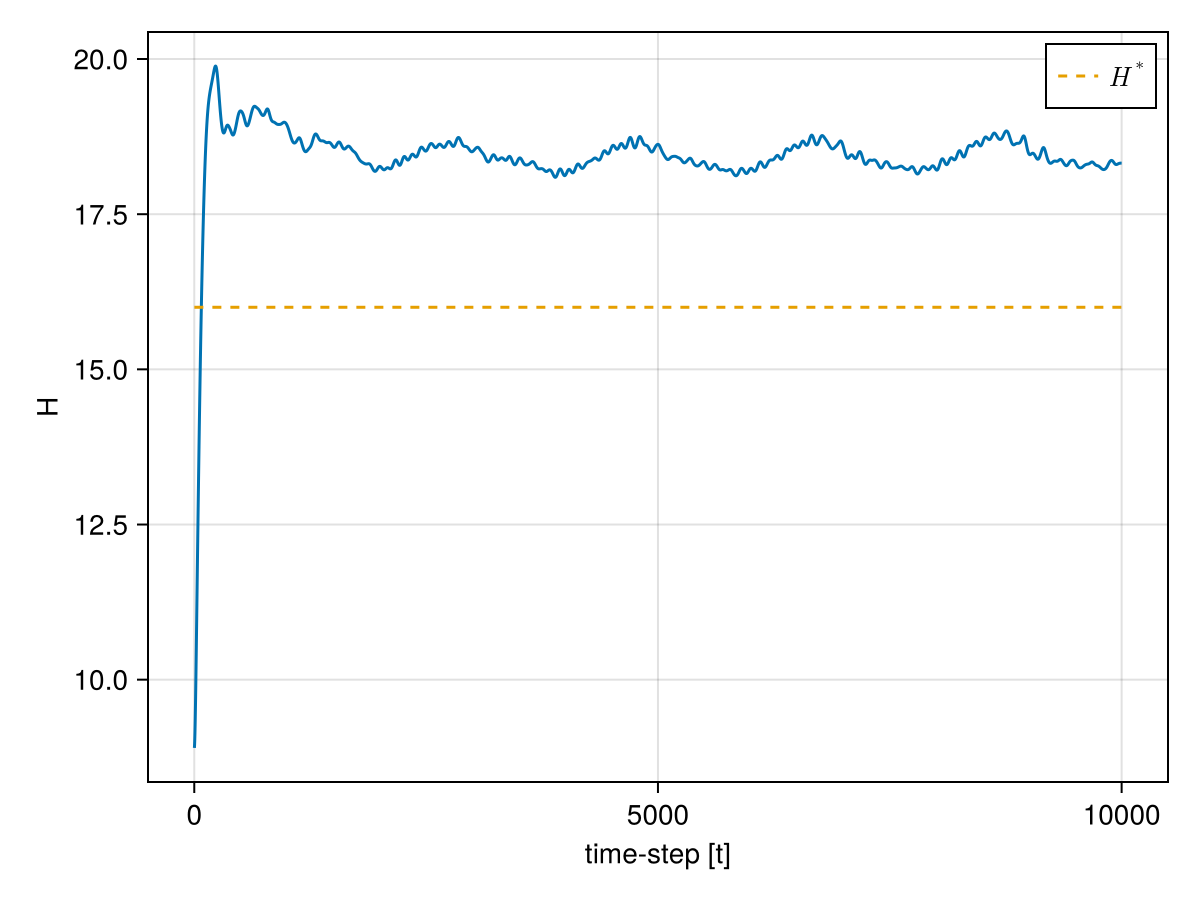
\includegraphics[width=\linewidth]{figures/ch5_collective/H_cross2.png}
            \caption{Hamiltonian $H$ over time}
            \label{plot:cross2_h}
        \end{subfigure}
        \begin{subfigure}{.49\textwidth}
            \centering
            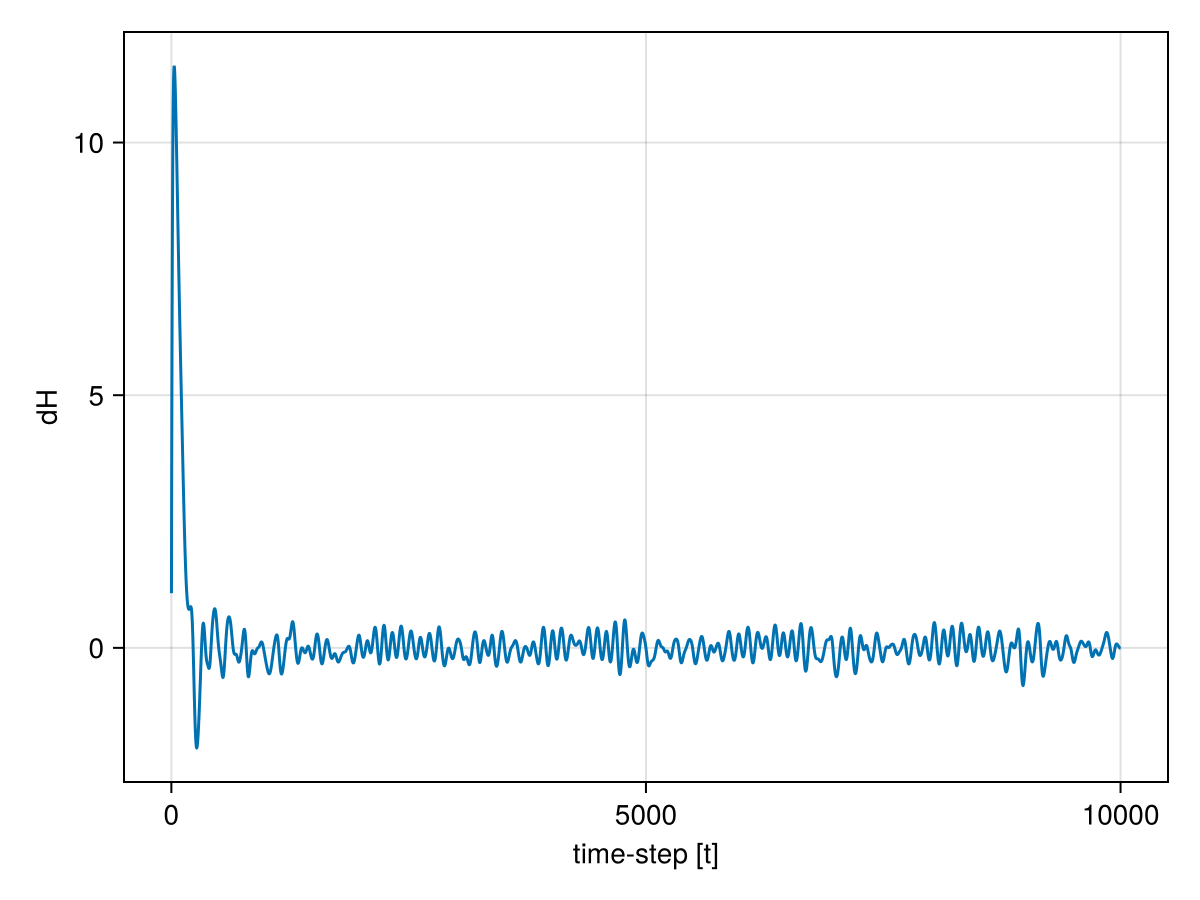
\includegraphics[width=\linewidth]{figures/ch5_collective/dH_cross2.png}
            \caption{$\frac{d}{dt}H$ over time}
            \label{plot:cross2_dh}
        \end{subfigure}
        \caption{Hamiltonian for cross flow with stripe formation with $\lambda = 2$}
        \label{plot:cross2_hamiltonian}
    \end{figure}



This is also apparent when we look at the plots for the Hamiltonian, as both the Hamiltonian periodically fluctuates over time and $\frac{d}{dt}H$ fluctuates about zero. However, the long term dynamics of the pedestrians would result in an arrangement where the pedestrians don't deviate from their desired directions, as shown in the next case.

    \item \textbf{Stripe Formation for cross flow with $\lambda = 3$}
    \begin{figure}[H]
        \centering
        \begin{subfigure}{0.49\textwidth}
            \centering
            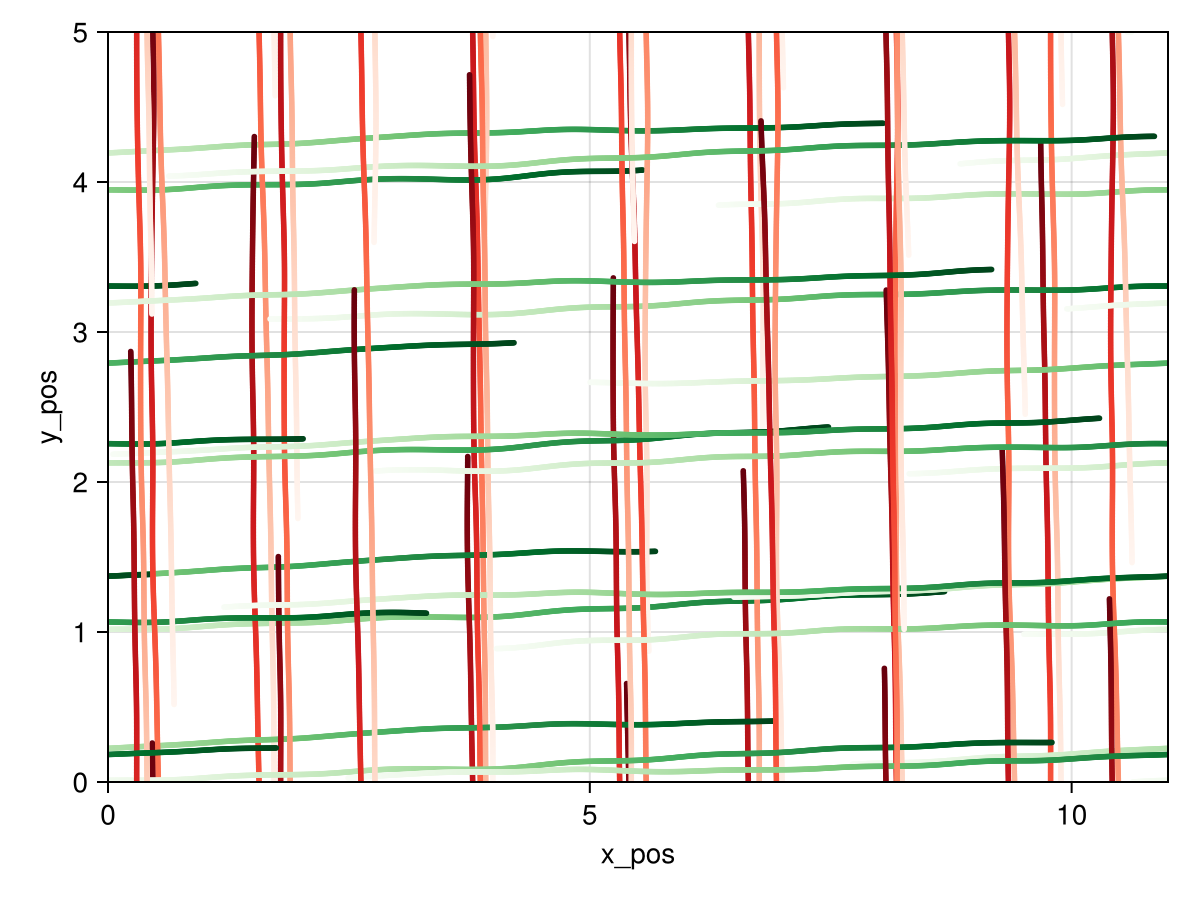
\includegraphics[width=\linewidth]{figures/ch5_collective/s0crossleap3flow_10000.png}
            \caption{Pedestrian trajectories}
            \label{plot:cross3_traj}
        \end{subfigure}
        \begin{subfigure}{.49\textwidth}
            \centering
            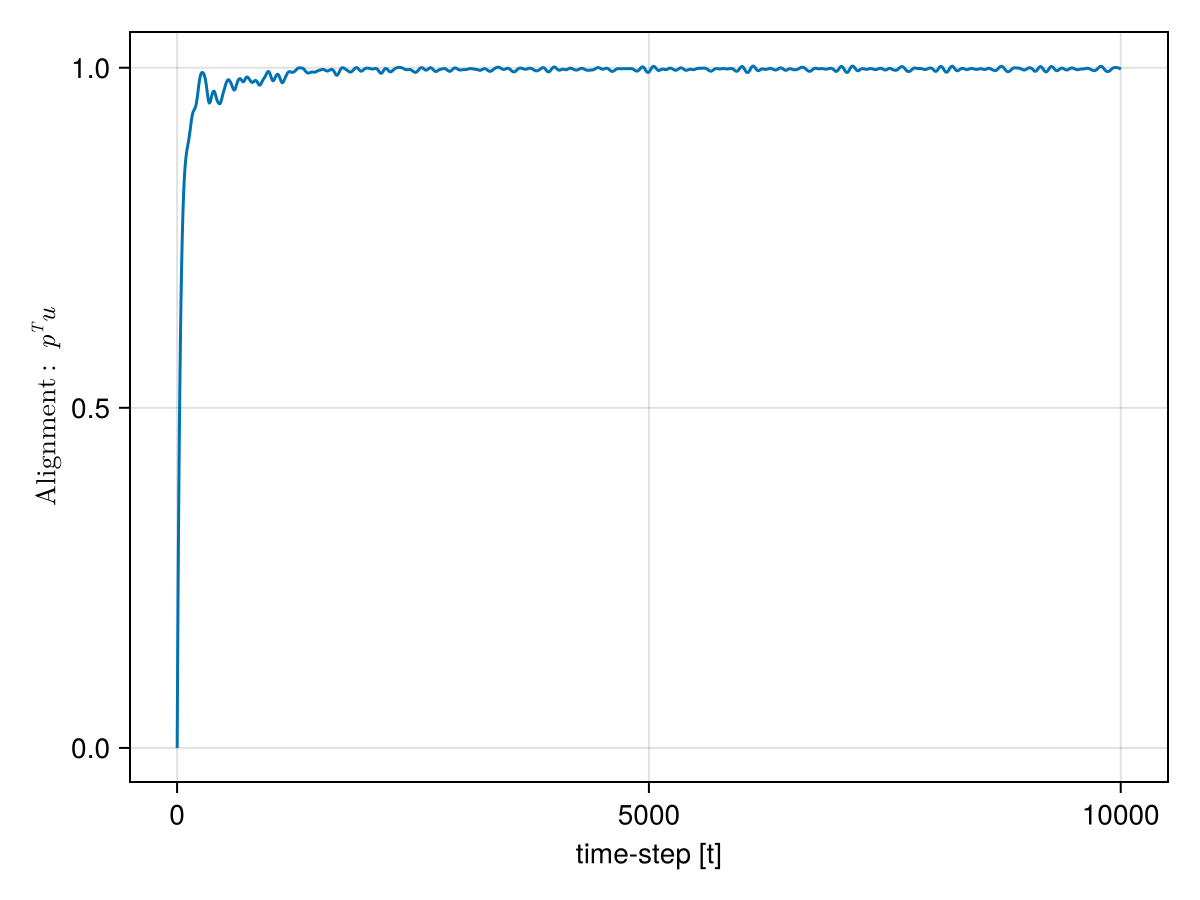
\includegraphics[width=\linewidth]{figures/ch5_collective/straight_cross3.png}
            \caption{Alignment}
            \label{plot:cross3_alignment}
        \end{subfigure}
        \caption{Improved stripe formation for cross flow with $\lambda = 3$}
        \label{plot:cross3}
    \end{figure}
Here we replicate the model from before, though we set $\lambda$ to a higher value, we can clearly observe a better stripe formation. The alignment also shows an improvement, as the value is closer to 1 than before, indicating that this stripe formation is an improvement from the previous case.

    \begin{figure}[H]
        \centering
        \begin{subfigure}{.49\textwidth}
            \centering
            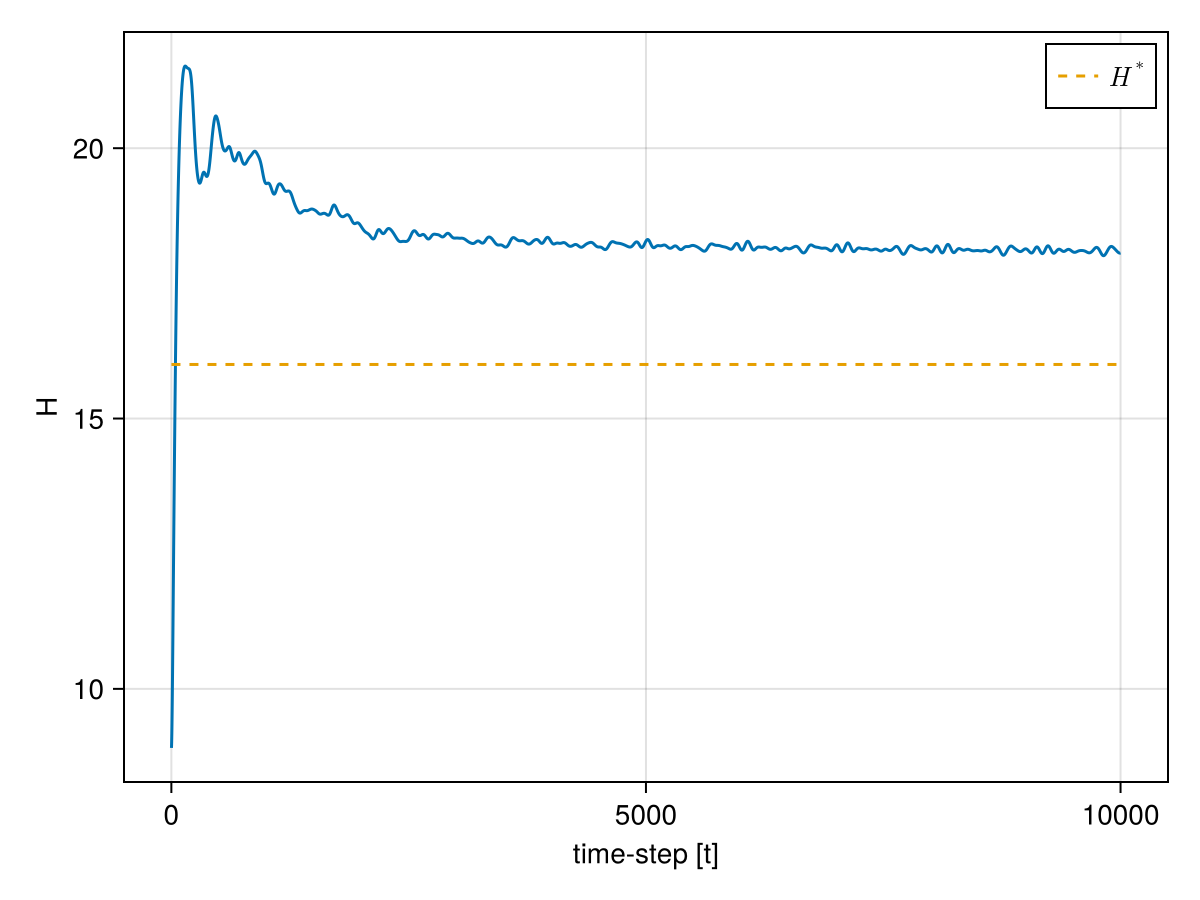
\includegraphics[width=\linewidth]{figures/ch5_collective/H_cross3.png}
            \caption{Hamiltonian $H$ over time}
            \label{plot:cross3_h}
        \end{subfigure}
        \begin{subfigure}{.49\textwidth}
            \centering
            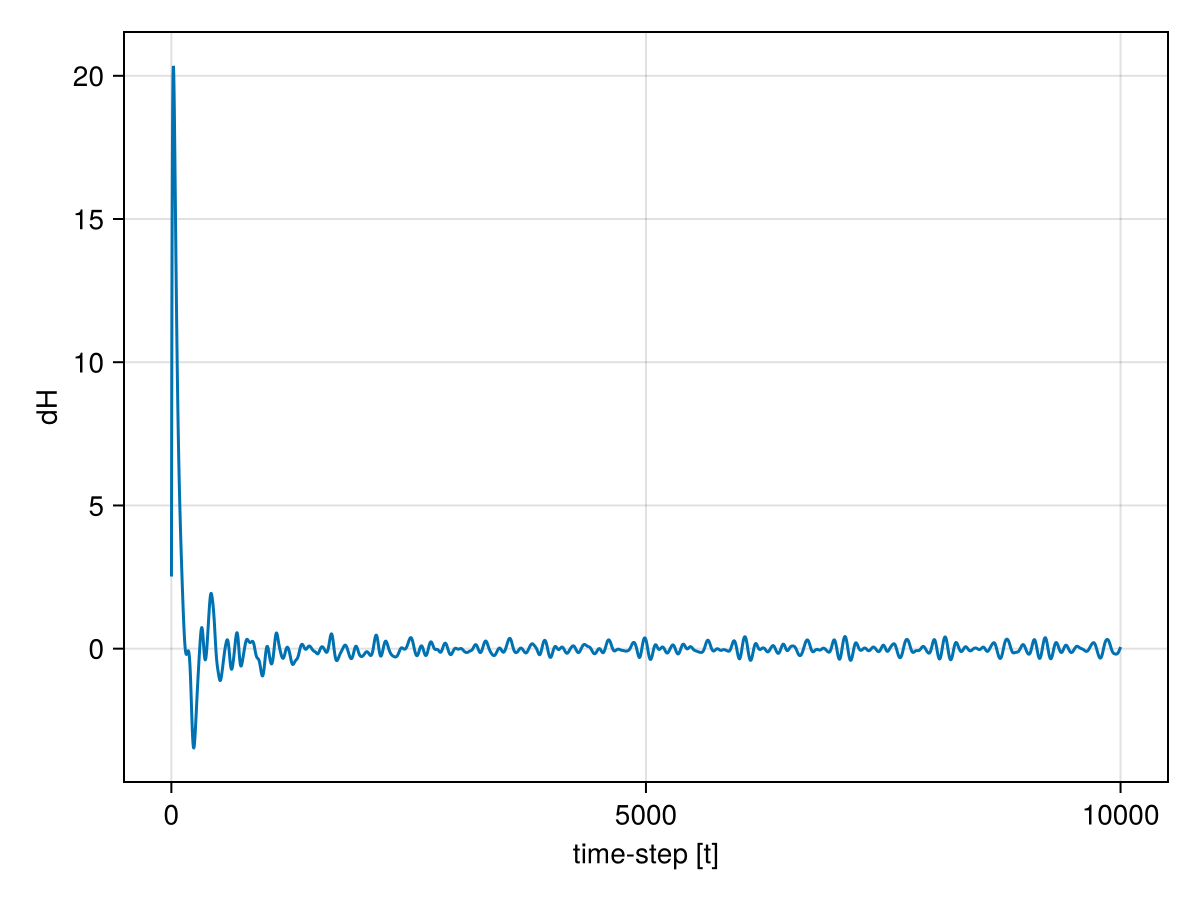
\includegraphics[width=\linewidth]{figures/ch5_collective/dH_cross3.png}
            \caption{$\frac{d}{dt}H$ over time}
            \label{plot:cross3_dh}
        \end{subfigure}
        \caption{Hamiltonian for cross flow with lane formation with $\lambda = 3$}
        \label{plot:cross3_hamiltonian}
    \end{figure}

The Hamiltonian as well as its derivative also don't fluctuate too much as $\frac{d}{dt}H$ decreases more quickly. In both of these cases, we can observe that the stripe formation occurs, and the Hamiltonian remains above $H^*$.

    \item \textbf{Gridlock for cross flow with $\lambda = 0.2$}
    \begin{figure}[H]
        \centering
        \begin{subfigure}{0.49\textwidth}
            \centering
            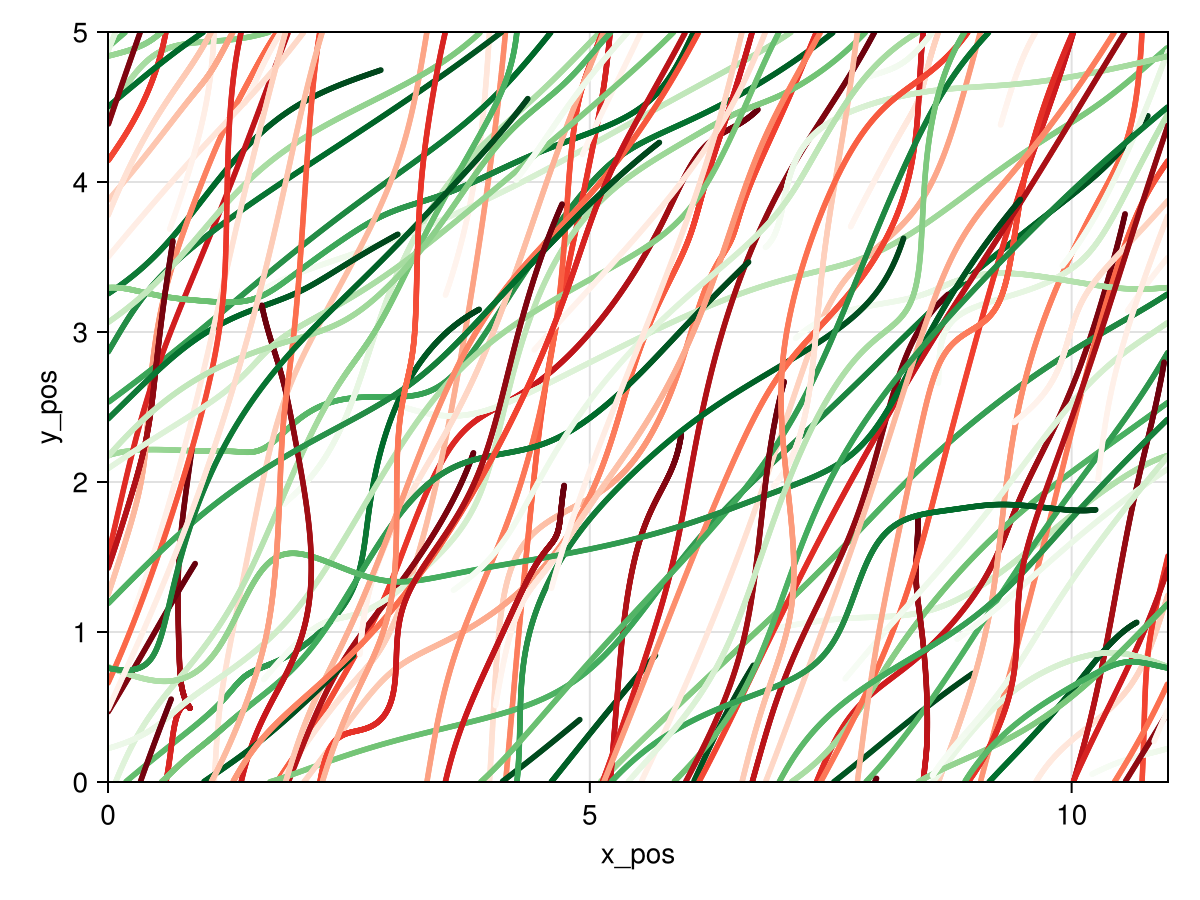
\includegraphics[width=\linewidth]{figures/ch5_collective/cross_gridlockdflow_4000.png}
            \caption{Pedestrian trajectories}
            \label{plot:crossgridlock_traj}
        \end{subfigure}
        \begin{subfigure}{.49\textwidth}
            \centering
            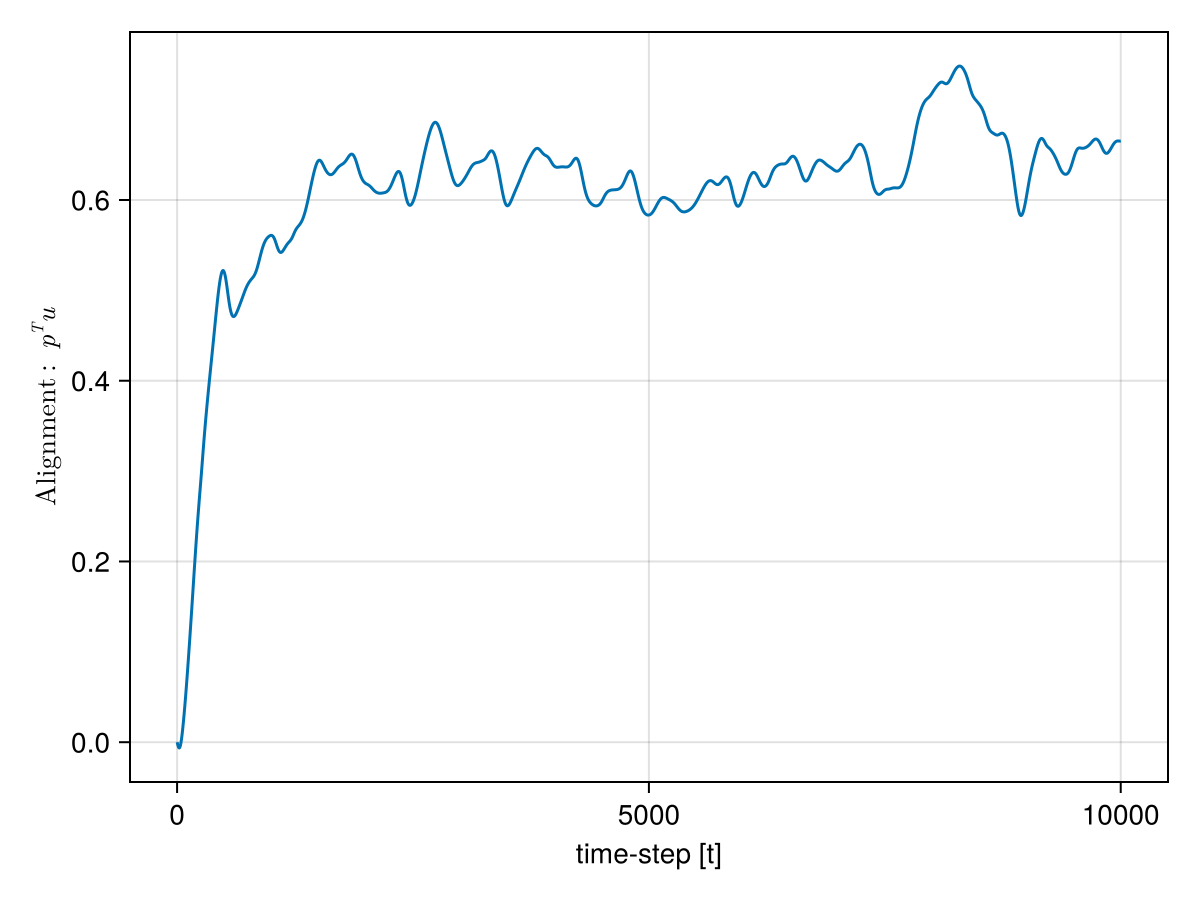
\includegraphics[width=\linewidth]{figures/ch5_collective/straight_gridlock_cross.png}
            \caption{Alignment}
            \label{plot:crossgridlock_alignment}
        \end{subfigure}
        \caption{Gridlock for cross flow}
        \label{plot:crossgridlock}
    \end{figure}
Here we can see that no stripe formation occurs, as $\lambda$ is not high enough for the pedestrians to be reactive. The alignment fluctuates and remains far below 1. The Hamiltonian also remain below $H^*$
\end{itemize}

    \begin{figure}[H]
        \centering
        \begin{subfigure}{.49\textwidth}
            \centering
            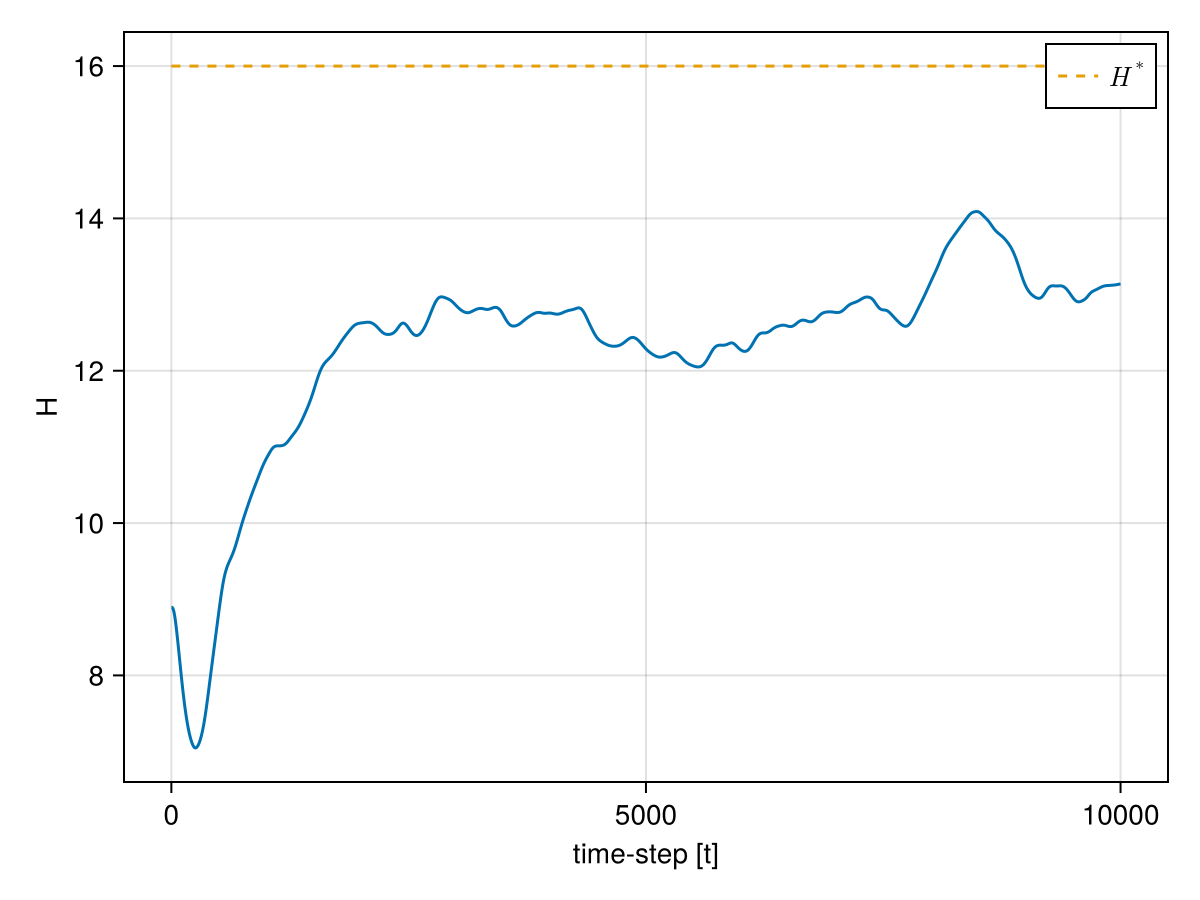
\includegraphics[width=\linewidth]{figures/ch5_collective/H_gridlock_cross.png}
            \caption{Hamiltonian $H$ over time}
            \label{plot:crossgridlock_h}
        \end{subfigure}
        \begin{subfigure}{.49\textwidth}
            \centering
            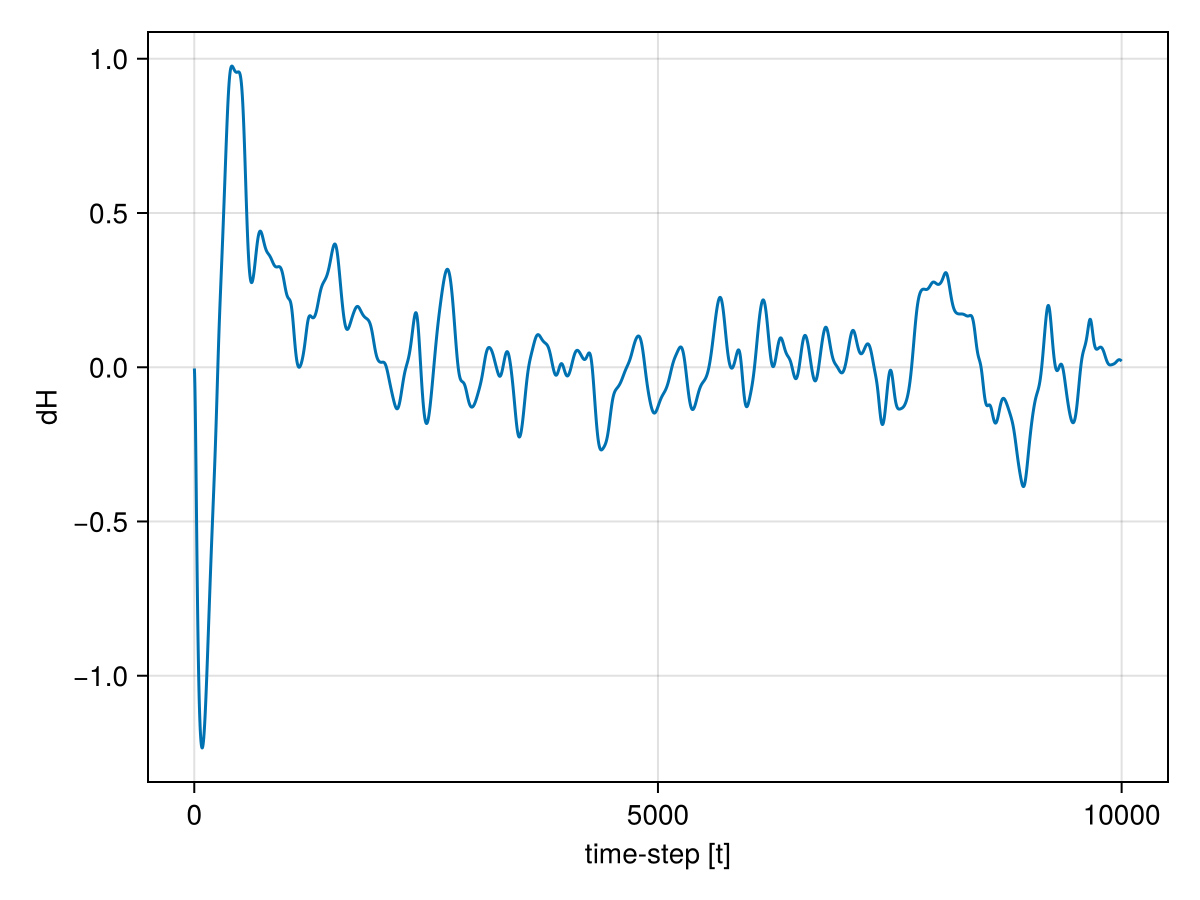
\includegraphics[width=\linewidth]{figures/ch5_collective/dH_gridlock_cross.png}
            \caption{$\frac{d}{dt}H$ over time}
            \label{plot:crossgridlock_dh}
        \end{subfigure}
        \caption{Hamiltonian for cross flow with gridlock}
        \label{plot:crossgridlock_hamiltonian}
    \end{figure}


From the simulations above, we have observed that collective dynamics occur when the Hamiltonian remains stable and above $H^*$. We will test this idea further in the next section where we subject our model with stochastic elements.

\subsection{Basic Dynamics with Stochastic Elements}
In this section, we once again pay our attention to the stochastic model dynamics, and simulate the model with basic dynamics as before with addition of stochastic elements. From a physical sense, one can interpret the addition of noise as 'warming' the system, and hence we will notice, for most cases, that the overall energy of the systems increase with increase in noise. We observe the long term dynamics, the Hamiltonian, and also its stochastic derivative $\d H$ over time. We also compare the dynamics of the stochastic (non-deterministic) system $\sigma \geq 0$ with their respective deterministic case $\sigma = 0$.
\begin{itemize}
    \item \textbf{No desired velocity $u_i = \begin{bmatrix} 0 & 0 \end{bmatrix}$ with $\lambda > 0$ and $\sigma \geq 0$}
    \begin{figure}[H]
        \centering
        \begin{subfigure}{.49\textwidth}
            \centering
            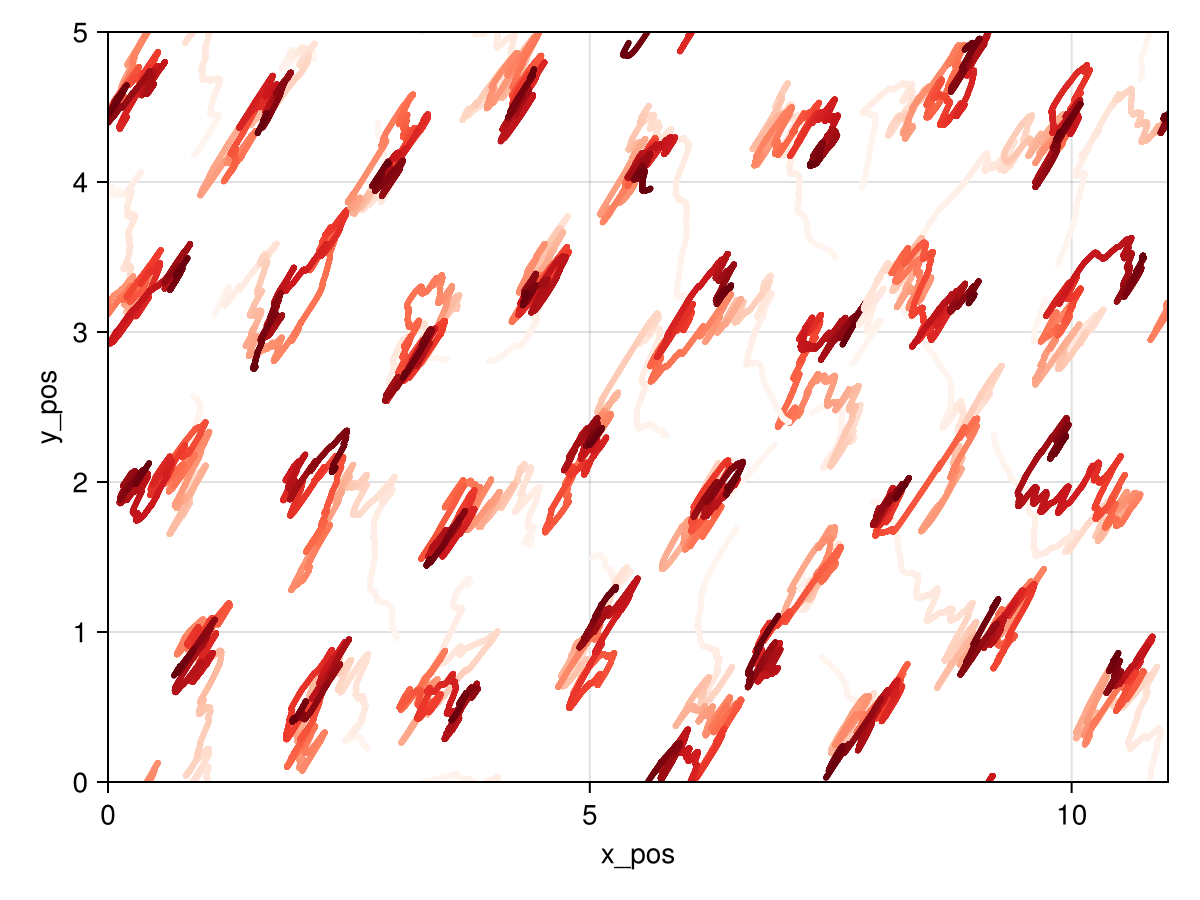
\includegraphics[width=\linewidth]{figures/ch5_basic_stoch/traj_stochastic_crys_10000.png}
            \caption{Pedestrian trajectories for $\sigma = 0.2$}
            \label{plot:stoc_crys_traj}
        \end{subfigure}
        \begin{subfigure}{.49\textwidth}
            \centering
            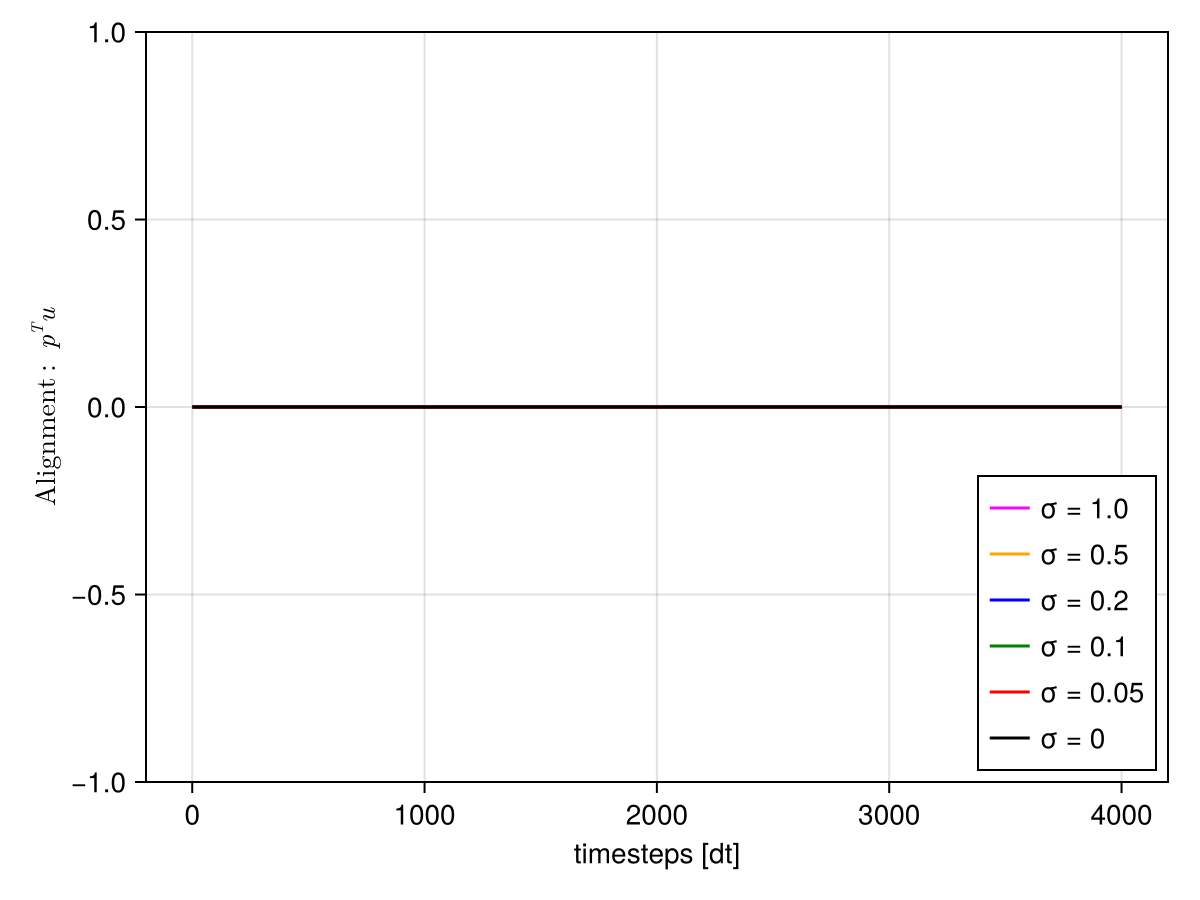
\includegraphics[width=\linewidth]{figures/ch5_basic_stoch/align_stochastic_crys.png}
            \caption{Alignment}
            \label{plot:stoc_crys_alignment}
        \end{subfigure}
        \caption{Crystallization with stochastic effects}
        \label{plot:stoc_crys}
    \end{figure}
Starting the same position as before, the pedestrians fluctuate about their positions with no clear direction as $u_i = 0$. Because of the dissipation parameter, the order of magnitude of the velocities with which the pedestrians fluctuate doesn't blow out of proportions, in contrast to the next case. The alignment, of course remain zero, as the pedestrians have no direction to align themselves to.

    \begin{figure}[H]
        \centering
        \begin{subfigure}{.49\textwidth}
            \centering
            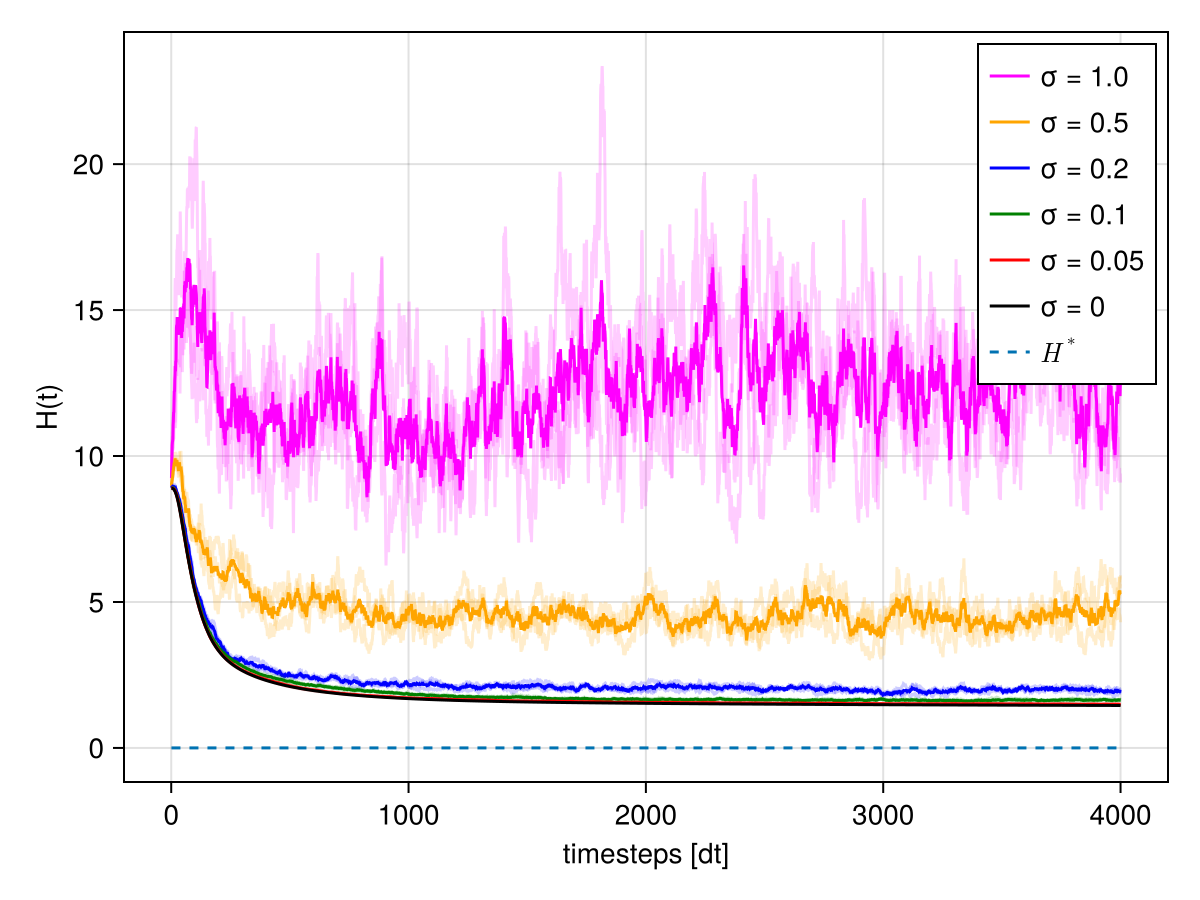
\includegraphics[width=\linewidth]{figures/ch5_basic_stoch/H_stochasic_crys.png}
            \caption{Hamiltonian $H$ over time}
            \label{plot:stoc_crys_h}
        \end{subfigure}
        \begin{subfigure}{.49\textwidth}
            \centering
            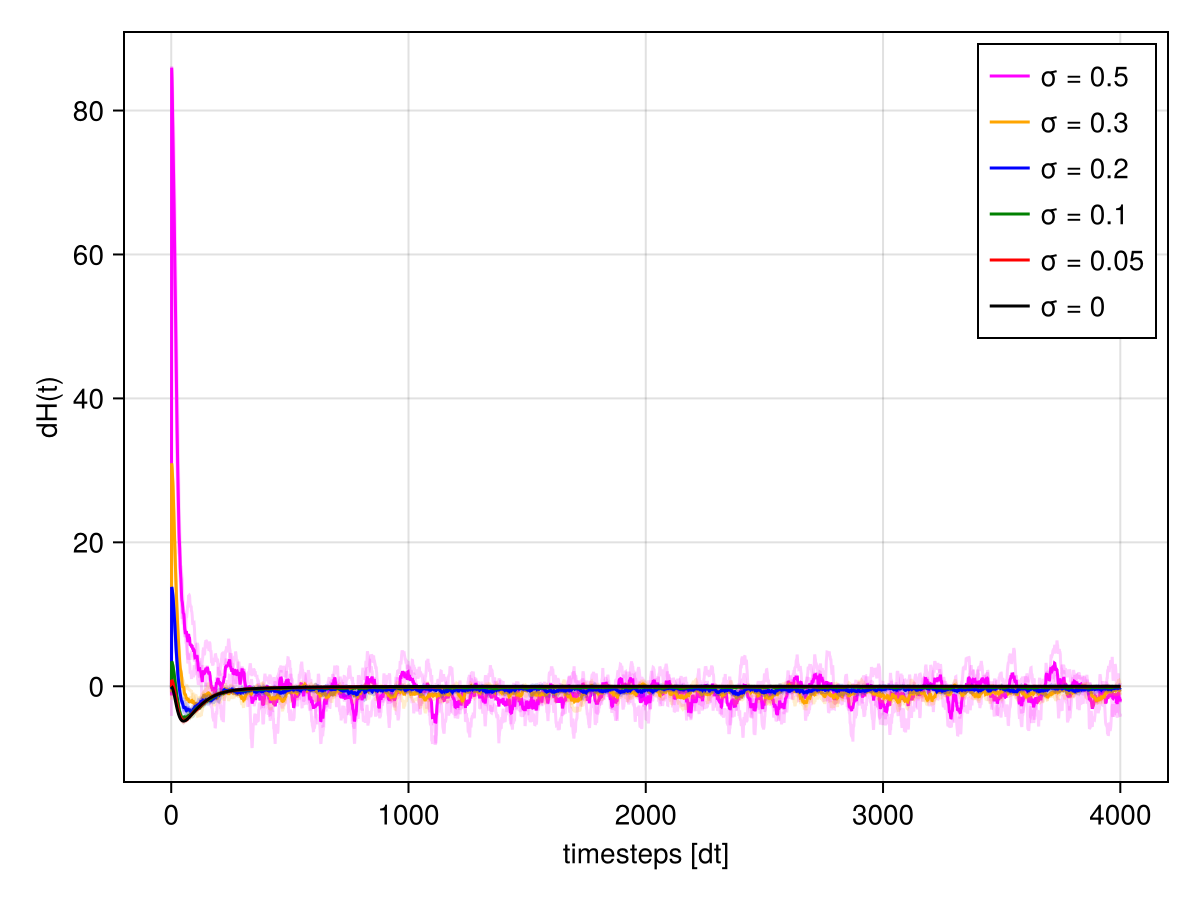
\includegraphics[width=\linewidth]{figures/ch5_basic_stoch/dH_stochasic_crys.png}
            \caption{$\d H$ over time}
            \label{plot:stoc_crys_dh}
        \end{subfigure}
        \caption{Hamiltonian under $u_i = 0$ and $\lambda > 0$ with stochastic effects}
        \label{plot:stoc_crys_hamiltonian}
    \end{figure}
It can be clearly seen that the Hamiltonian in all cases $\sigma \geq 0$ remains above $H^*$ and fluctuates about a constant line, indicating that dissipation occurs, and that the system energy does not diverge to higher values.

    \item \textbf{No dissipation ($\lambda = 0$) with $\sigma \geq 0$}
    \begin{figure}[H]
        \centering
        \begin{subfigure}{.49\textwidth}
            \centering
            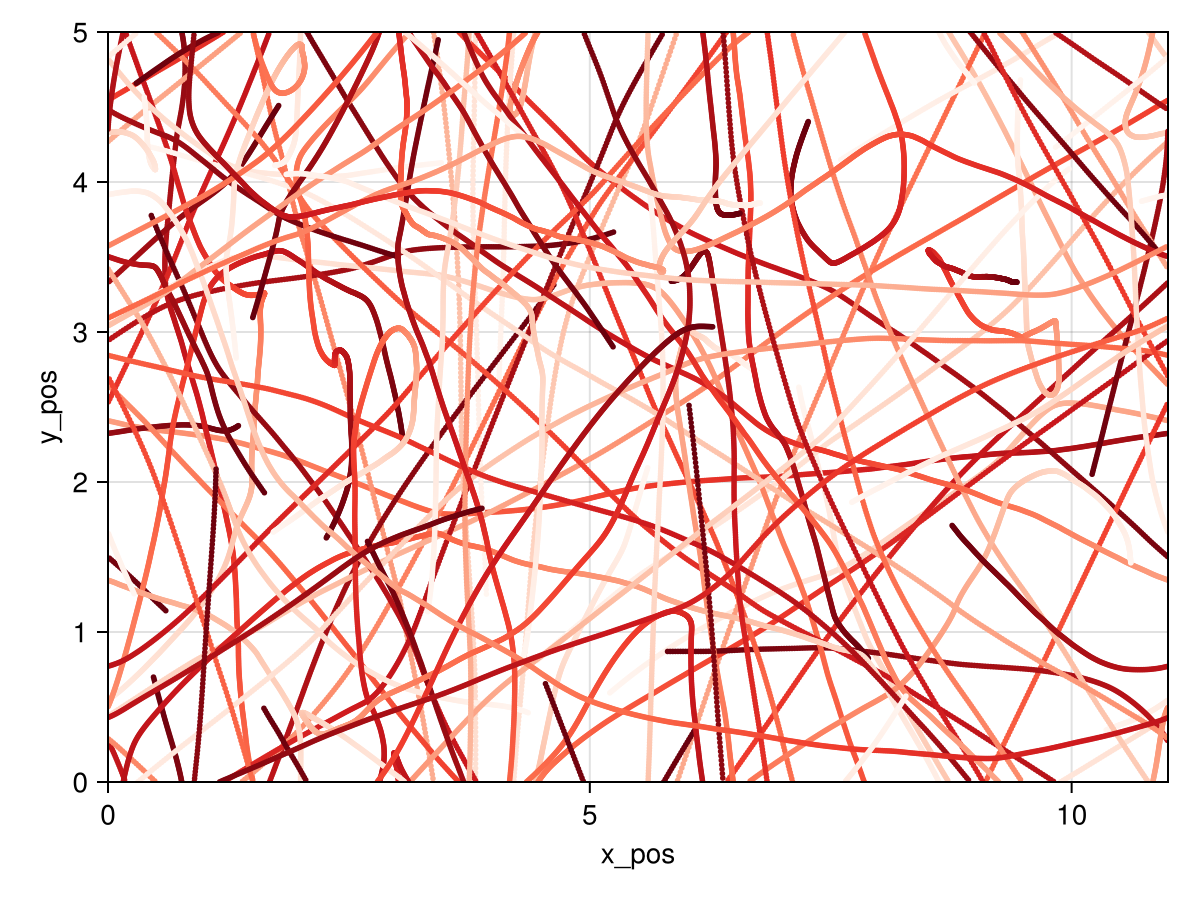
\includegraphics[width=\linewidth]{figures/ch5_basic_stoch/traj_stochastic_nodisp_10000.png}
            \caption{Pedestrian trajectories for $\sigma = 0.2$}
            \label{plot:stoc_nodisp_traj}
        \end{subfigure}
        \begin{subfigure}{.49\textwidth}
            \centering
            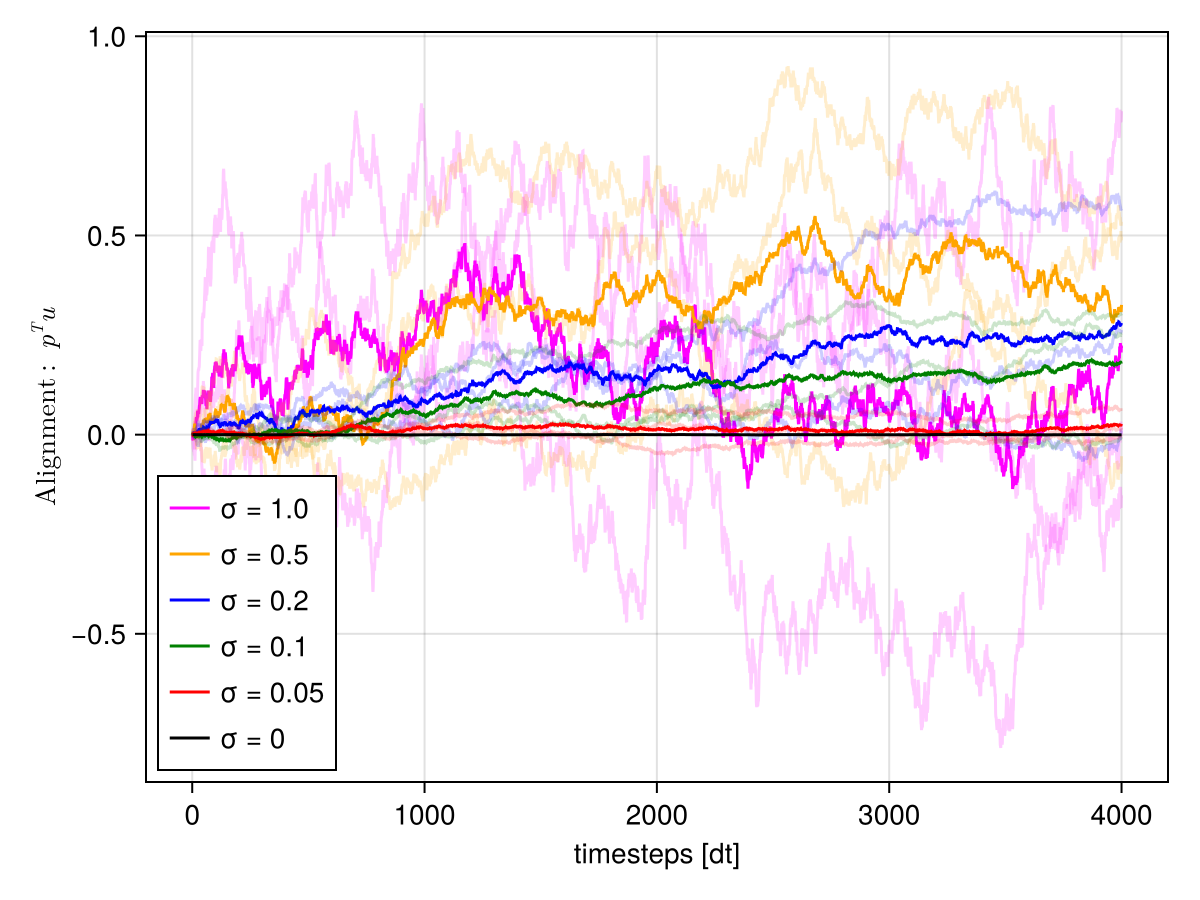
\includegraphics[width=\linewidth]{figures/ch5_basic_stoch/align_stochastic_nodisp.png}
            \caption{Alignment}
            \label{plot:stoc_nodisp_alignment}
        \end{subfigure}
        \caption{Trajectories of pedestrians in a non-dissipative system with stochastic effects}
        \label{plot:stoc_nodisp}
    \end{figure}
Here, with no dissipation, we witness the warming effects due to noise. The system gains energy and remains closed, the velocities of the pedestrians will keep increasing. The system remains disordered as the pedestrians fail to align themselves with their desired velocities, as indicated by the alignment being near 0 and rapidly fluctuating.
    \begin{figure}[H]
        \centering
        \begin{subfigure}{.49\textwidth}
            \centering
            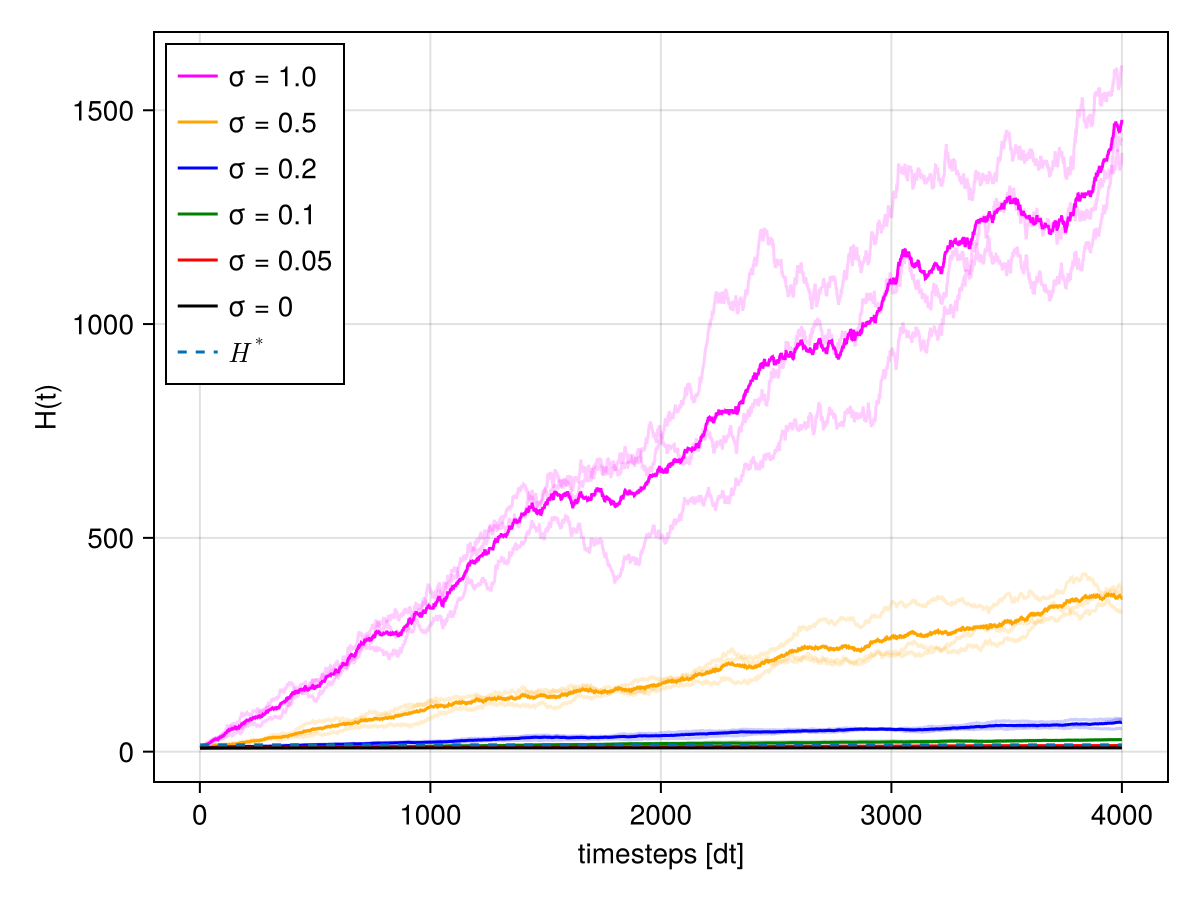
\includegraphics[width=\linewidth]{figures/ch5_basic_stoch/H_stochasic_nodisp.png}
            \caption{Hamiltonian $H$ over time}
            \label{plot:stoc_nodisp_h}
        \end{subfigure}
        \begin{subfigure}{.49\textwidth}
            \centering
            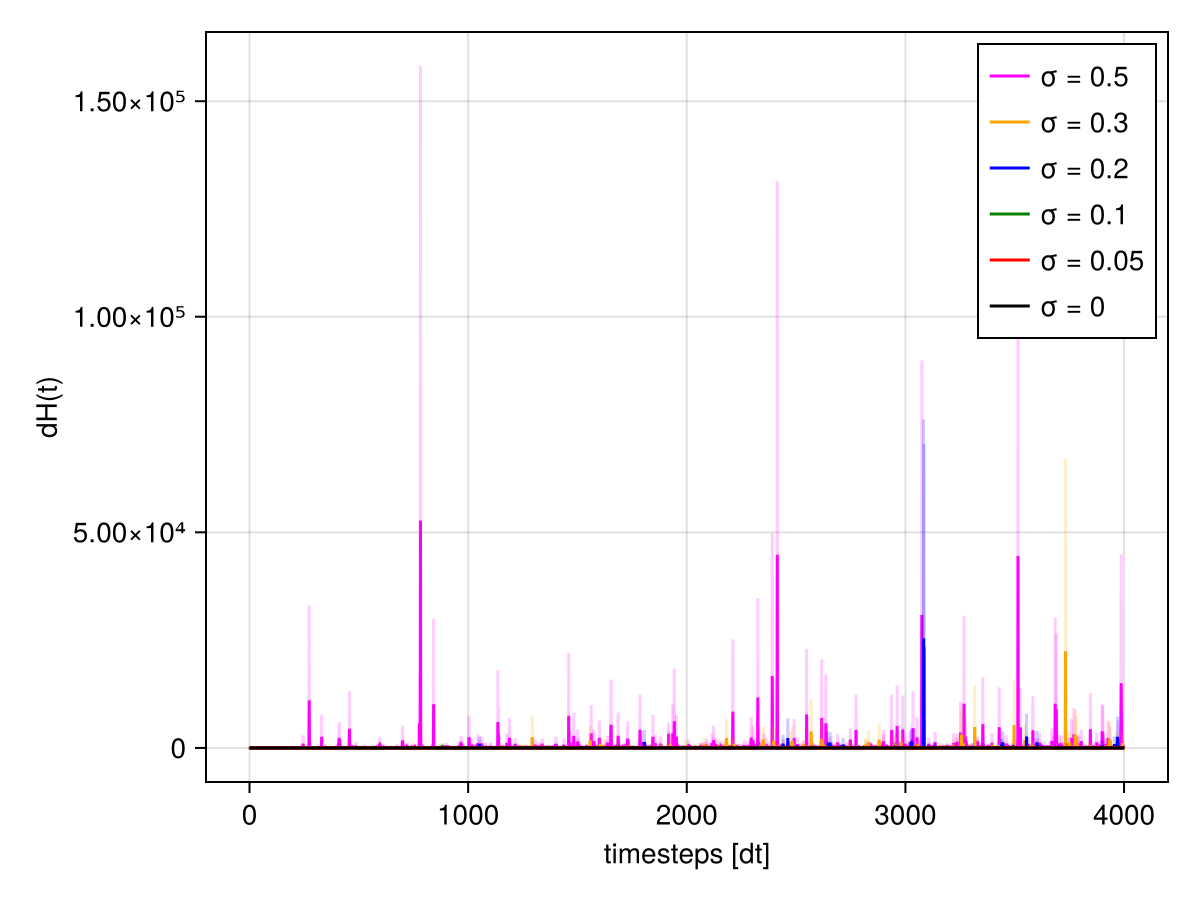
\includegraphics[width=\linewidth]{figures/ch5_basic_stoch/dH_stochasic_nodisp.png}
            \caption{$\d H$ over time}
            \label{plot:stoc_nodisp_dh}
        \end{subfigure}
        \caption{Hamiltonian under non-dissipative system with stochastic effects}
        \label{plot:stoc_nodisp_hamiltonian}
    \end{figure}

As the system gains energy without dissipation, the Hamiltonian diverges to higher values.
    \item \textbf{No interaction ($A = 0$) with $u_i = \begin{bmatrix} 1 & 0 \end{bmatrix}$ and $\sigma \geq 0$}
    \begin{figure}[H]
        \centering
        \begin{subfigure}{.49\textwidth}
            \centering
            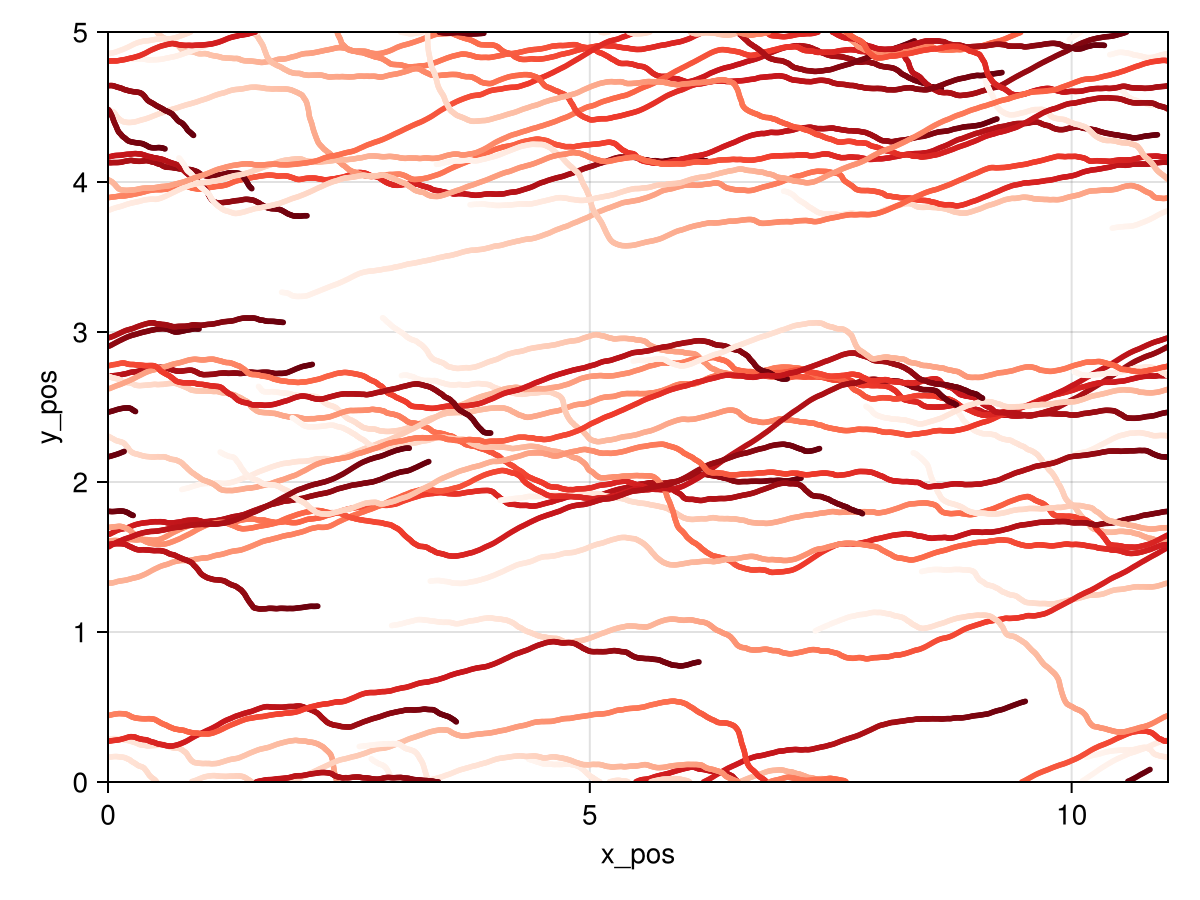
\includegraphics[width=\linewidth]{figures/ch5_basic_stoch/traj_stochastic_nointeraction_10000.png}
            \caption{Pedestrian trajectories for $\sigma = 0.5$}
            \label{plot:stoc_nointeraction_traj}
        \end{subfigure}
        \begin{subfigure}{.49\textwidth}
            \centering
            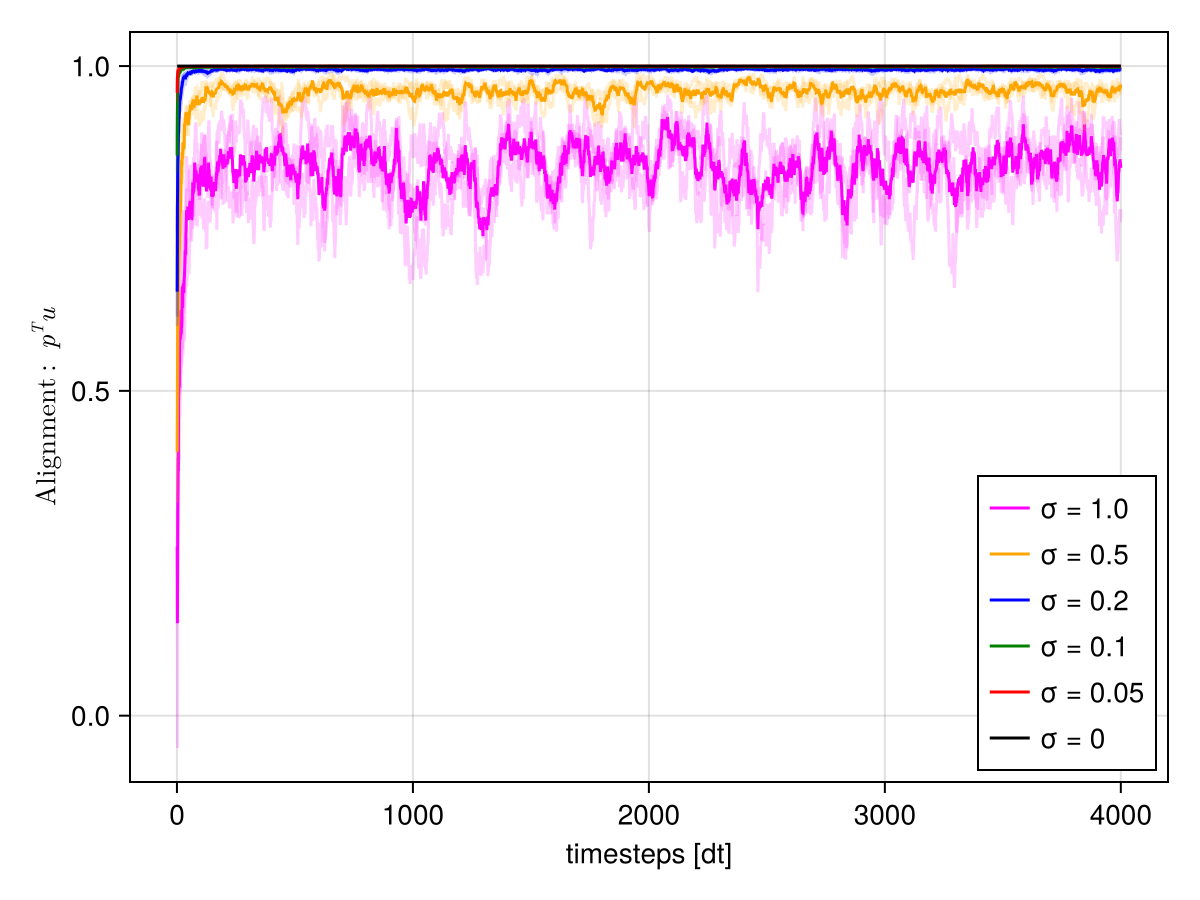
\includegraphics[width=\linewidth]{figures/ch5_basic_stoch/align_stochastic_nointeraction.png}
            \caption{Alignment}
            \label{plot:stoc_nointeraction_alignment}
        \end{subfigure}
        \caption{Pedestrian trajectories with no interaction and stochastic effects}
        \label{plot:stoc_nointeraction}
    \end{figure}
Recall the deterministic counterpart with no interaction with other the pedestrians \autoref{plot:nointeraction}, the pedestrians were able to reach their desired velocities as soon as the simulation starts. However, here, with the addition of noise, we witness a clear transition from ordered to disordered trajectories due to the volatility $\sigma$. This is also indicated in the alignment, as the system remains very near 1 for values below $\sigma \leq 0.2$, beyond this value the trajectories, however, are disrupted. 

    \begin{figure}[H]
        \centering
        \begin{subfigure}{.49\textwidth}
            \centering
            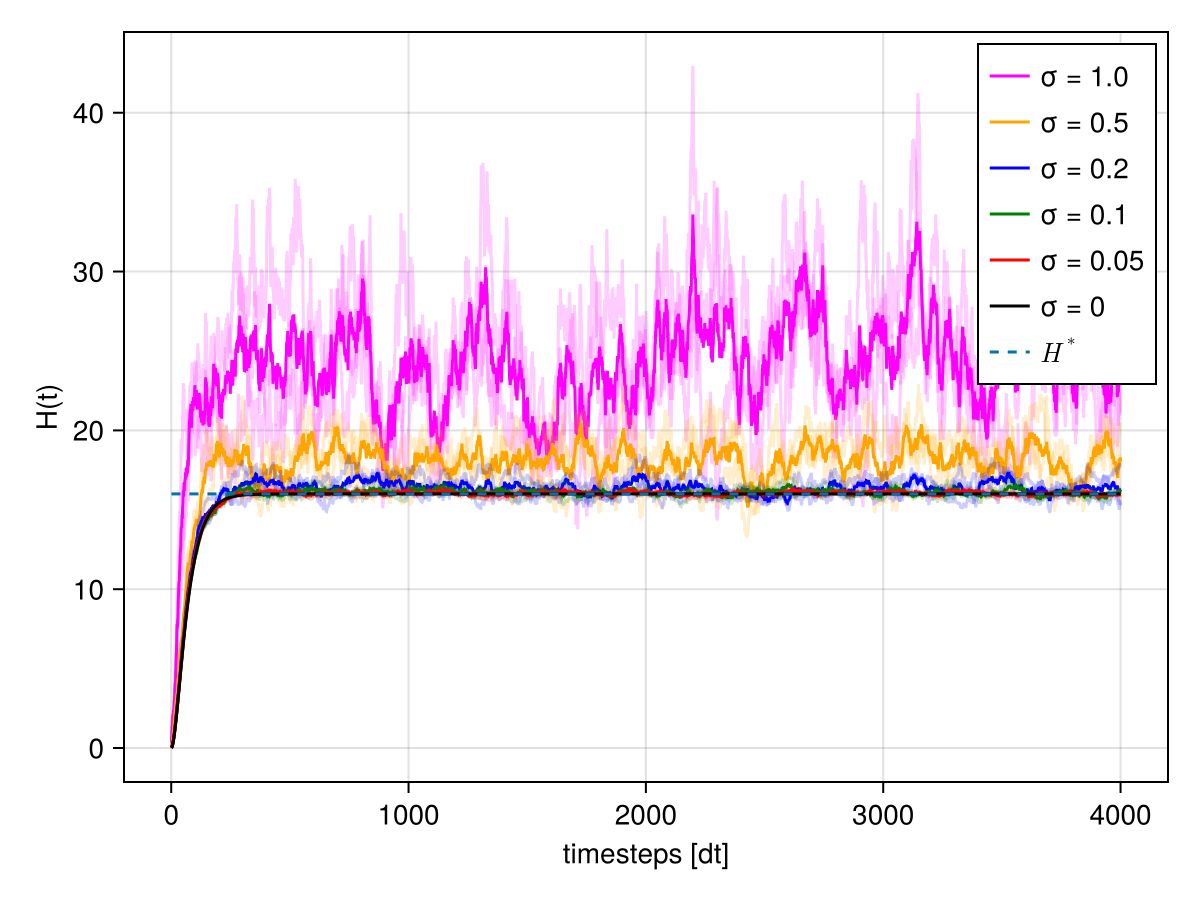
\includegraphics[width=\linewidth]{figures/ch5_basic_stoch/H_stochasic_nointeraction.png}
            \caption{Hamiltonian $H$ over time}
            \label{plot:stoc_nointeraction_h}
        \end{subfigure}
        \begin{subfigure}{.49\textwidth}
            \centering
            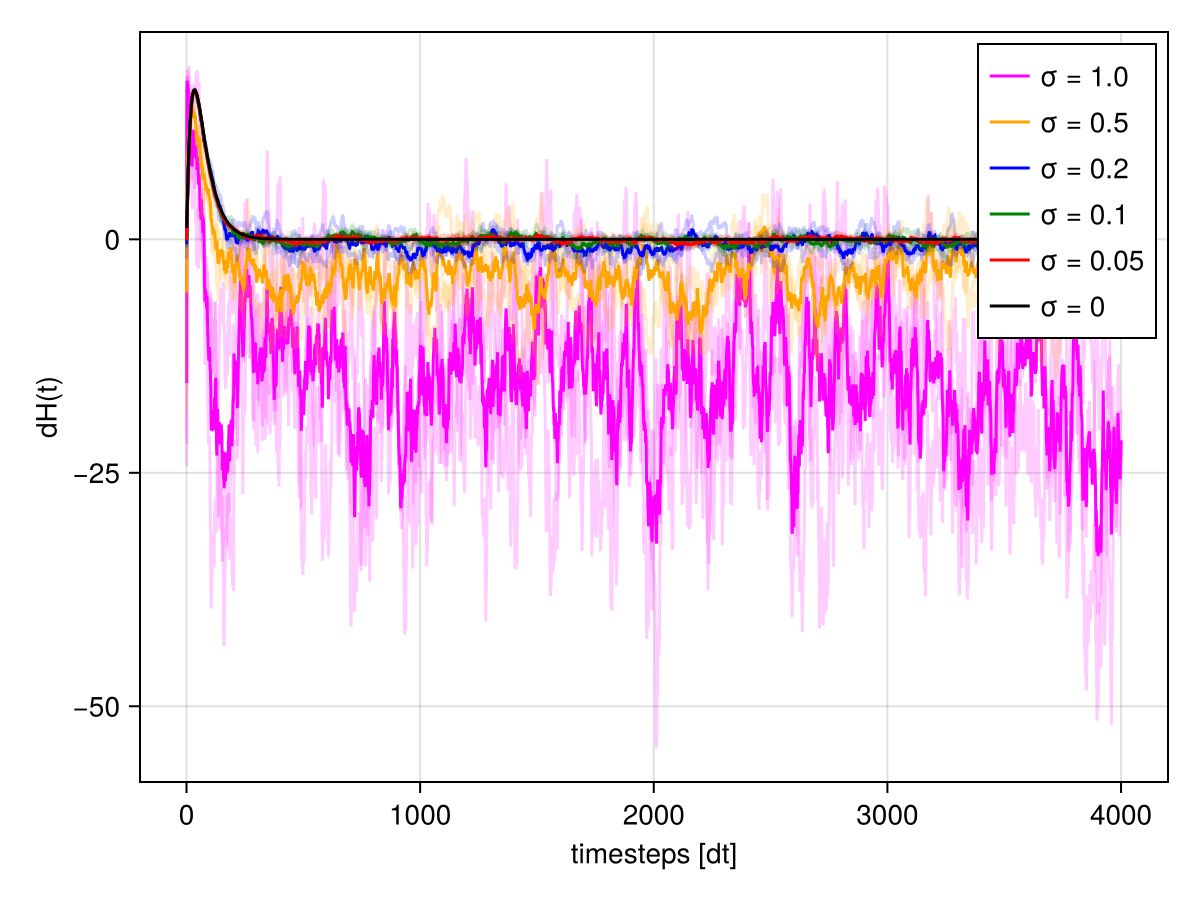
\includegraphics[width=\linewidth]{figures/ch5_basic_stoch/dH_stochasic_nointeraction.png}
            \caption{$\d H$ over time}
            \label{plot:stoc_nointeraction_dh}
        \end{subfigure}
        \caption{Hamiltonian under $A=0$ and stochastic effects}
        \label{plot:stoc_nointeraction_hamiltonian}
    \end{figure}
The Hamiltonian also indicates orderly system behavior for $\sigma \leq 0.2$, as the plots remains at or above $H^*$ and fluctuate only a little, however for values $\sigma \geq 0.5$, the system devolves into disorder as it can be witnessed by the rapid fluctuations in the Hamiltonian.
    \item \textbf{Unidirectional flow ($\sigma \geq 0$)}
    \begin{figure}[H]
        \centering
        \begin{subfigure}{.49\textwidth}
            \centering
            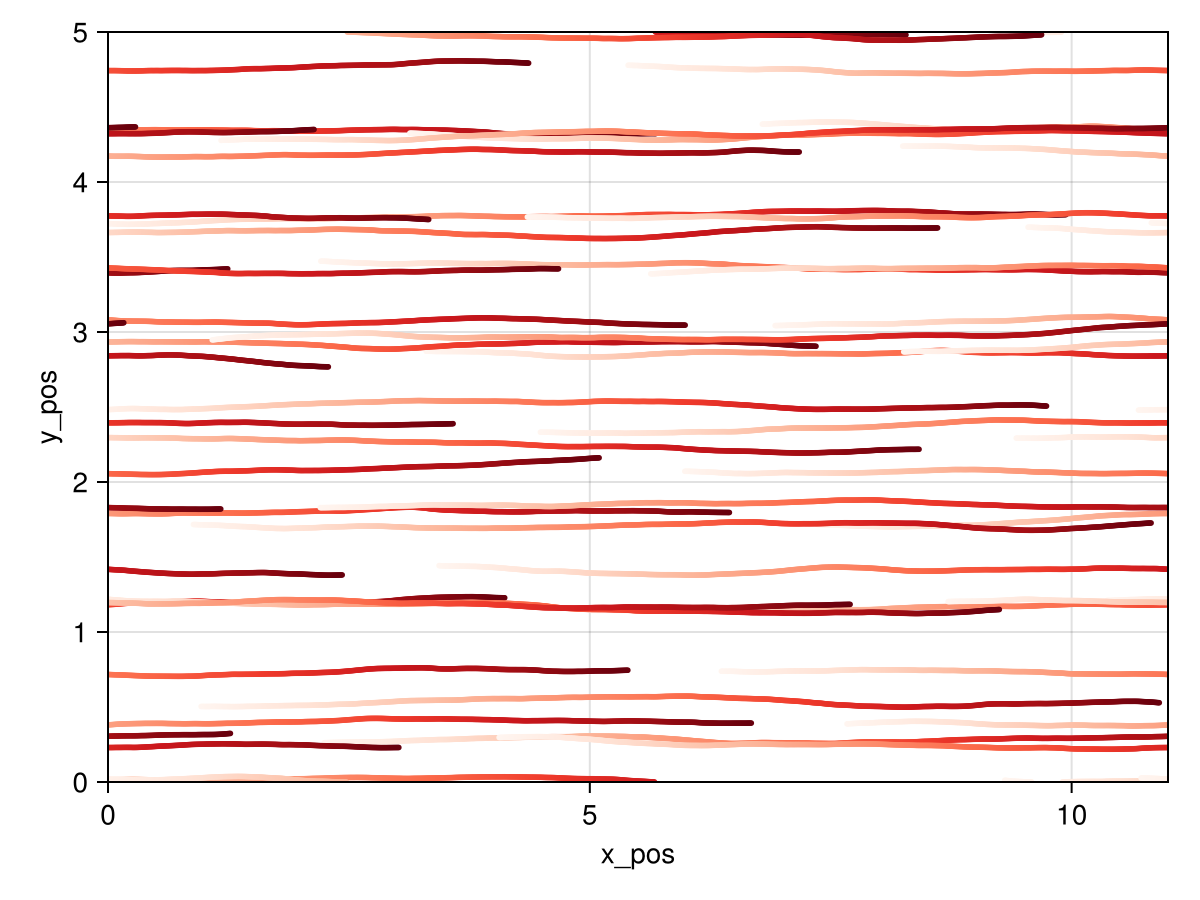
\includegraphics[width=\linewidth]{figures/ch5_collective_stoch/traj_stochastic_uni_10000.png}
            \caption{Pedestrian trajectories for $\sigma = 0.05$}
            \label{plot:stoc_uni_traj}
        \end{subfigure}
        \begin{subfigure}{.49\textwidth}
            \centering
            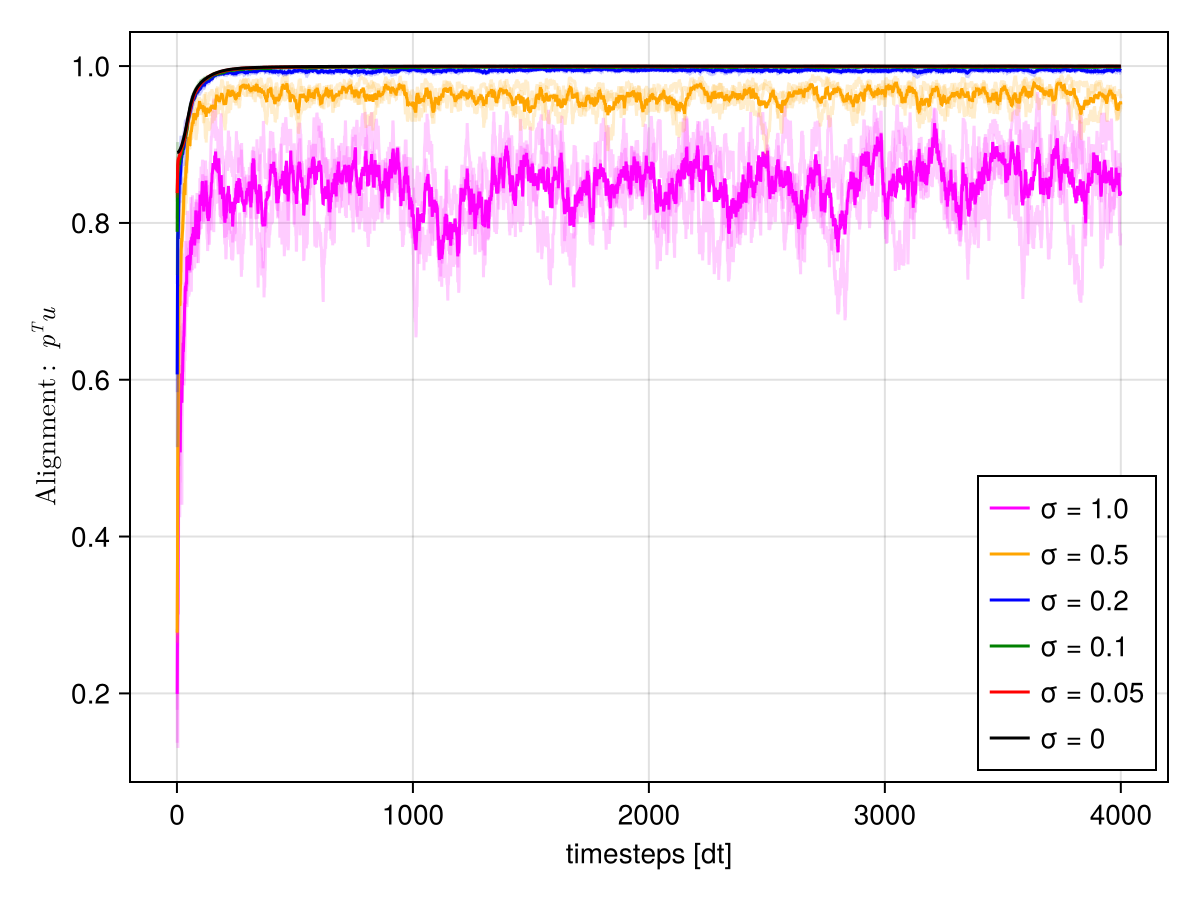
\includegraphics[width=\linewidth]{figures/ch5_collective_stoch/align_stochastic_uni.png}
            \caption{Alignment}
            \label{plot:stoc_uni_alignment}
        \end{subfigure}
        \caption{Unidirectional flow with stochastic effects}
        \label{plot:stoc_uni}
    \end{figure}
    We can observe that increasing the volatility $\sigma$ in the dynamics perturbs the velocity of the pedestrians in the unidirectional case. The effects of the randomness are as expected; the dynamics deviate more when the volatility is high. The alignment indicates that the system dynamics remain ordered for lower values of $\sigma$.

    \begin{figure}[H]
        \centering
        \begin{subfigure}{.49\textwidth}
            \centering
            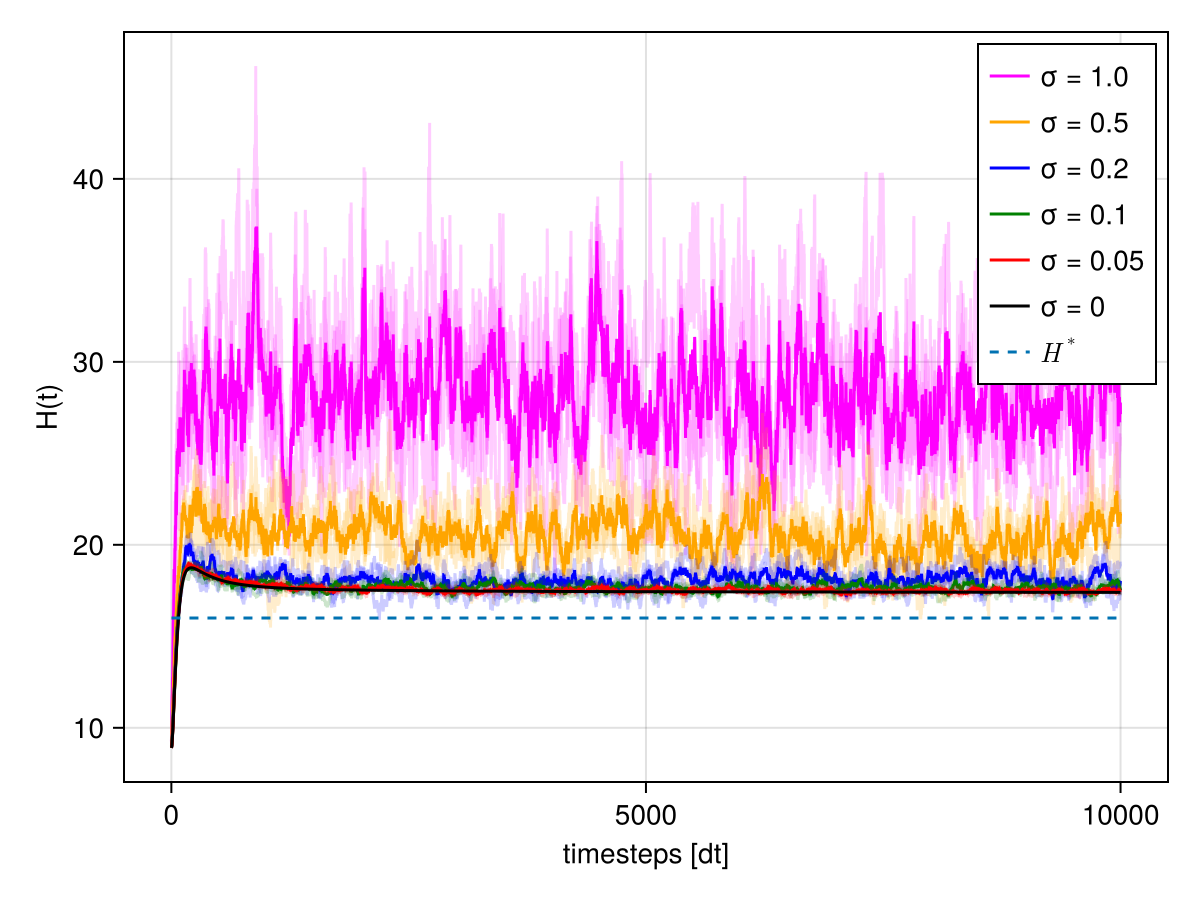
\includegraphics[width=\linewidth]{figures/ch5_collective_stoch/H_stochasic_uni.png}
            \caption{Hamiltonian $H$ over time}
            \label{plot:stoc_uni_h}
        \end{subfigure}
        \begin{subfigure}{.49\textwidth}
            \centering
            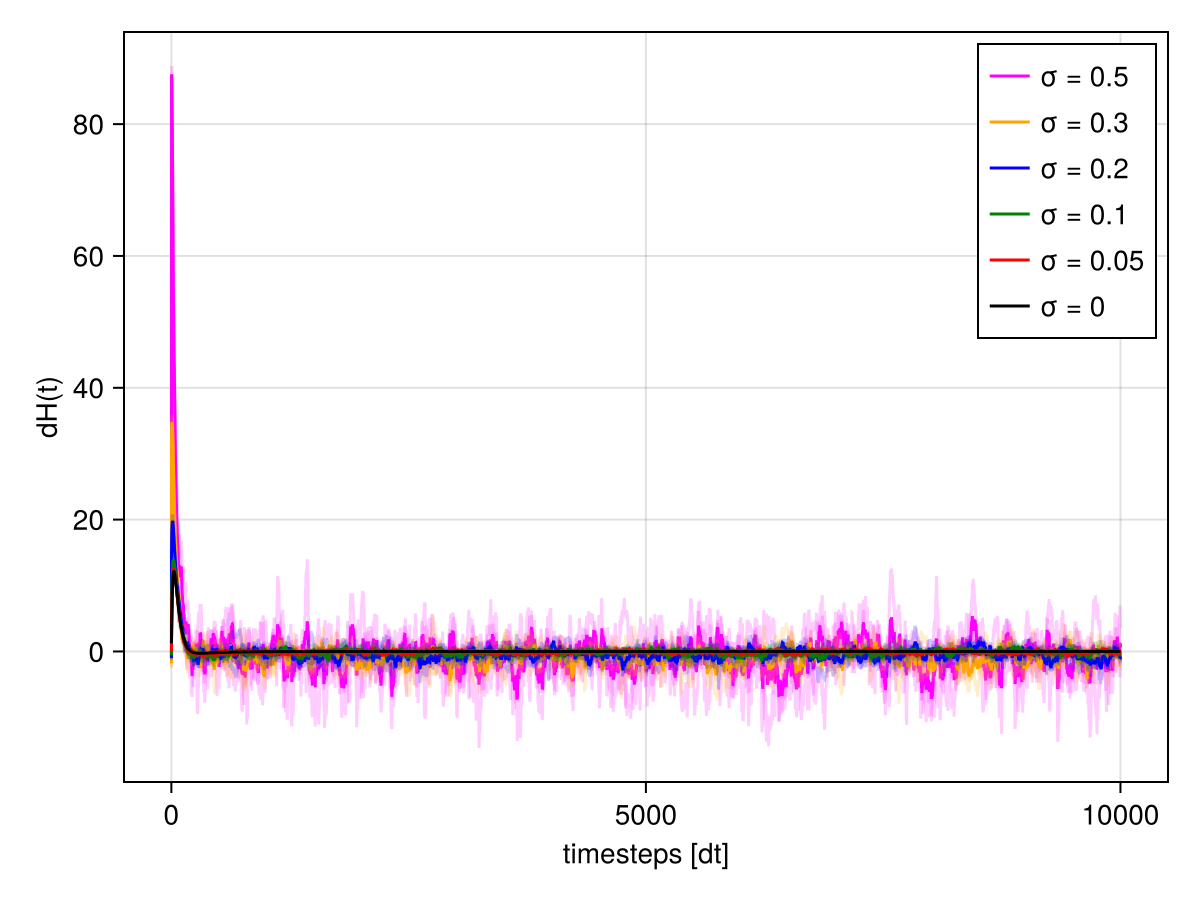
\includegraphics[width=\linewidth]{figures/ch5_collective_stoch/dH_stochasic_uni.png}
            \caption{$\d H$ over time}
            \label{plot:stoc_uni_dh}
        \end{subfigure}
        \caption{Hamiltonian for unidirectional flow with stochastic effects}
        \label{plot:stoc_uni_hamiltonian}
    \end{figure}

The Hamiltonian is the least for cases where there is no noise, indicating that the pedestrians are able to reach their desired velocities without perturbations, however with higher volatility the system becomes disordered as indicated via the rapid fluctuations in the Hamiltonian.

\end{itemize}


% \pagebreak

\subsection{Collective Dynamics with Stochastic Effects}
We will keep the same parameters as \autoref{code:model_init}, and focus mainly on counter and cross flows with addition of stochastic effects.

\begin{itemize}
    \item \textbf{Cross flow ($\sigma \geq 0$)}
    \begin{figure}[H]
        \centering
        \begin{subfigure}{.49\textwidth}
            \centering
            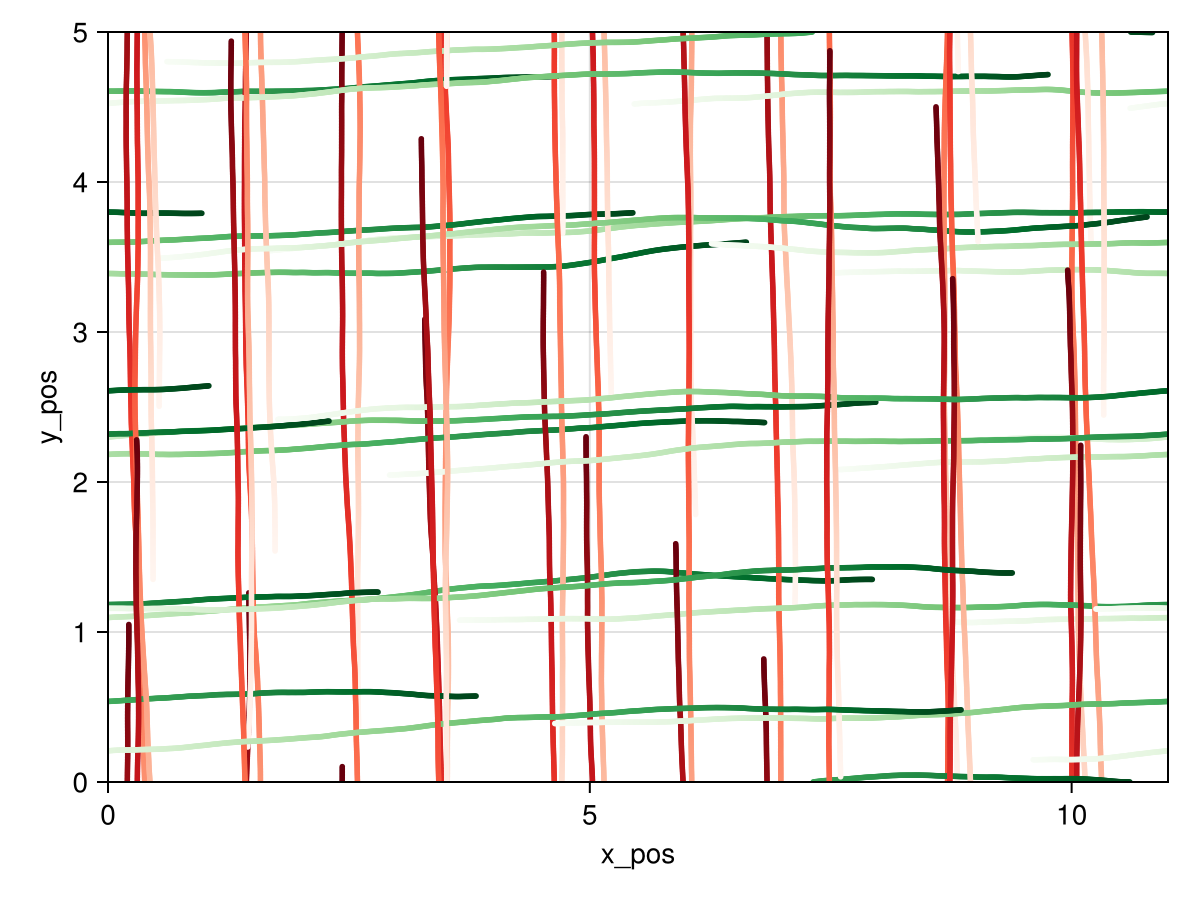
\includegraphics[width=\linewidth]{figures/ch5_collective_stoch/traj_stochastic_cross_10000.png}
            \caption{Pedestrian trajectories for $\sigma = 0.05$}
            \label{plot:stoc_cross_traj}
        \end{subfigure}
        \begin{subfigure}{.49\textwidth}
            \centering
            \includegraphics[width=\linewidth]{figures/ch5_collective_stoch/align_stochastic_cross.png}
            \caption{Alignment}
            \label{plot:stoc_cross_alignment}
        \end{subfigure}
        \caption{Cross flow with stochastic effects}
        \label{plot:stoc_cross}
    \end{figure}
    For cross flows, the stochastic dynamics produce interesting results. It can be seen from the trajectories as well as the alignment that the stripe formation is improved in contrast to its deterministic counterpart from \autoref{plot:cross2}. Upon closer inspection, we can see that the alignment for cases $\sigma \leq 0.2$ is much closer to 1 than that for $\sigma = 0$.
    
    \begin{figure}[H]
        \centering
        \begin{subfigure}{.49\textwidth}
            \centering
            \includegraphics[width=\linewidth]{figures/ch5_collective_stoch/H_stochasic_cross.png}
            \caption{Hamiltonian $H$ over time}
            \label{plot:stoc_cross_h}
        \end{subfigure}
        \begin{subfigure}{.49\textwidth}
            \centering
            \includegraphics[width=\linewidth]{figures/ch5_collective_stoch/dH_stochasic_cross.png}
            \caption{$\d H$ over time}
            \label{plot:stoc_cross_dh}
        \end{subfigure}
        \caption{Hamiltonian for cross flows with stochastic effects}
        \label{plot:stoc_cross_hamiltonian}
    \end{figure}
This phenomenon is made even more apparent when look at the Hamiltonian, for small positive values of $\sigma$, the Hamiltonian is even less than the deterministic case. For values $\sigma \leq 0.2$, as indicated in \cite{khelfa2021initiating}, the trajectories of the pedestrians also show that the stripe formation is improved with the addition of noise in contrast to its deterministic counterpart \autoref{plot:cross2}. This counterintuitive phenomenon for the stochastic cross flow is known as 'noise-induced ordering' \cite{d2021canard}. However, this stripe formation is disrupted with increase in noise, particularly for values $\sigma \geq 0.5$
    \item \textbf{Counter flow ($\sigma \geq 0$)}
    \begin{figure}[H]
        \centering
        \begin{subfigure}{.49\textwidth}
            \centering
            \includegraphics[width=\linewidth]{figures/ch5_collective_stoch/traj_stochastic_counter_10000.png}
            \caption{Pedestrian trajectories for $\sigma = 0.2$}
            \label{plot:stoc_counter_traj}
        \end{subfigure}
        \begin{subfigure}{.49\textwidth}
            \centering
            \includegraphics[width=\linewidth]{figures/ch5_collective_stoch/align_stochastic_counter.png}
            \caption{Alignment}
            \label{plot:stoc_counter_alignment}
        \end{subfigure}
        \caption{Counter flow with stochastic effects}
        \label{plot:stoc_counter}
    \end{figure}
    In the case of the counter flow, however, we do not see an improvement in lane formation with addition of noise in the system. The lane formation is perturbed with the increase in noise and becomes indistinguishable from disordered movement when $\sigma \geq 0.5$ as indicated both by the alignment and the Hamiltonian, signalling a phenomenon known as 'freezing by heating' \cite{helbing2000freezing}.

    \begin{figure}[H]
        \centering
        \begin{subfigure}{.49\textwidth}
            \centering
            \includegraphics[width=\linewidth]{figures/ch5_collective_stoch/H_stochasic_counter.png}
            \caption{Hamiltonian $H$ over time}
            \label{plot:stoc_counter_h}
        \end{subfigure}
        \begin{subfigure}{.49\textwidth}
            \centering
            \includegraphics[width=\linewidth]{figures/ch5_collective_stoch/dH_stochasic_counter.png}
            \caption{$\d H$ over time}
            \label{plot:stoc_counter_dh}
        \end{subfigure}
        \caption{Hamiltonian for counter flows with stochastic effects}
        \label{plot:stoc_counter_hamiltonian}
    \end{figure}

\end{itemize}

All the dynamics shown in this section have the overall Hamiltonian greater than $H^*$, but for values of $\sigma$, the Hamiltonian rapidly fluctuates and the conditions for self-organization are not met. Indicating erratic movement of the overall dynamics of the agents, resulting in no phase changes from disordered to ordered dynamics. However, for low values of $\sigma$, the self-organization is improved for cross flows, resulting in stripe formations that are better than that of the deterministic case.


